\documentclass[ 11pt]{article}
\usepackage[utf8]{inputenc}
\usepackage[a4paper,width=190mm,top=25mm,bottom=25mm]{geometry}
\usepackage{graphicx} 
\usepackage{amssymb}
\usepackage{booktabs,	 longtable, makecell}
\usepackage{multirow}

\graphicspath{{/home/azaiez/Documents/Cours/These/European Commission/Programs/Figures/}{/home/azaiez/Documents/Cours/These/European Commission/Programs/Figures/}}

\title{European Commission}
\author{}
\date{June 2023}

\begin{document}

\maketitle

Problem with 'S.A.' node. 
\section{Model using hypergraphs or graphs?}

\subsection{Hpyergraph}
Number of hyperedges : 11214\\
Number of entities (nodes): 4541\\
Number of edges in a bipartite graph 32501 \\
Mean cardinality : 2.90\\
Std cardinality : 2.25\\

- Correlation between centralities of hyperedges.\\

\begin{tabular}{lrrr}
\toprule
 & Betweenness & Closeness & Cardinality \\
\midrule
Betweenness & 1.000000 & 0.514992 & 0.732040 \\
Closeness & 0.514992 & 1.000000 & 0.397166 \\
Cardinality & 0.732040 & 0.397166 & 1.000000 \\
\bottomrule
\end{tabular}

     $\Rightarrow$  big hyperedges have a high cardinality
     
\subsection{Graph}
Number of entities (nodes): 4541\\
Number of edges : 35139 \\


\section{Centralities}
\subsection{Degree}

\subsection{Betweenness}

\subsection{Eigenvector}

\section{Correlation between E.U. grant and centralities}
restrict graph to organisation appearing the E.U. transparency register. \\
Number of nodes = 3637 \\
The network still connected \\
\begin{tabular}{|ccccc|}
\hline
             &Members FTE  &Eigenvector   & Degree  &Betweenness\\
E.U. Grants  &0.002598    &0.008545  &0.028295     &0.015429\\
\hline
\end{tabular}  \\
$\Rightarrow$ No significant correlation


\newpage
\begin{itemize}
 \item problem when downloading the data. The seperator ',' appears in organization name
  


\begin{tabular}{lrr}
\toprule
 & count & proportion \\
Category of registration &  &  \\
\midrule
Companies and groups & 1199 & 0.27 \\
Non-governmental organisations, platforms and networks and similar & 954 & 0.21 \\
Trade and business associations & 813 & 0.18 \\
NaN & 734 & 0.16 \\
Trade unions and professional associations & 237 & 0.05 \\
Think tanks and research institutions & 171 & 0.04 \\
Professional consultancies & 137 & 0.03 \\
Other organisations, public or mixed entities & 113 & 0.03 \\
Academic institutions & 79 & 0.02 \\
Associations and networks of public authorities & 42 & 0.01 \\
Organisations representing churches and religious communities & 15 & 0.00 \\
Law firms & 14 & 0.00 \\
Self-employed individuals & 9 & 0.00 \\
\bottomrule
\end{tabular}

\begin{tabular}{lrr}
\toprule
 & count & proportion \\
Country &  &  \\
\midrule
BELGIUM & 953 & 0.210934 \\
NaN & 734 & 0.162461 \\
GERMANY & 420 & 0.092961 \\
FRANCE & 346 & 0.076583 \\
NETHERLANDS & 274 & 0.060646 \\
UNITED STATES & 255 & 0.056441 \\
UNITED KINGDOM & 229 & 0.050686 \\
SPAIN & 140 & 0.030987 \\
ITALY & 129 & 0.028552 \\
FINLAND & 114 & 0.025232 \\
SWITZERLAND & 94 & 0.020806 \\
SWEDEN & 84 & 0.018592 \\
IRELAND & 81 & 0.017928 \\
AUSTRIA & 78 & 0.017264 \\
DENMARK & 78 & 0.017264 \\
POLAND & 71 & 0.015715 \\
CZECH REPUBLIC & 39 & 0.008632 \\
PORTUGAL & 39 & 0.008632 \\
LUXEMBOURG & 38 & 0.008411 \\
NORWAY & 34 & 0.007525 \\
\bottomrule
\end{tabular}



\end{itemize}





\newpage
\section{Orbis data base}
\begin{itemize}
	\item Problem with separators solved by scraping eu web sites
	\item Add director general meetings. Need to specify a minimal date above which meeting should be taken into account (2019 beginning  of the mandate)
	\item Match organization names with orbis detabase. Orbis keep the A scored matches + manual matching of the non-automatically matched.
	
	\item cleaning data : 
		\begin{itemize}
		\item in EU meeting, there are a few entities that have been mistyped. Use a dictionnary to search and replace these entities.
		\item Names with double spacing or " are not let unchanged with the orbis matching. This concerns 22 organization names.  Solved by manually restore the original names in the organization names files.  Export organization names i.xlsx
		\item drop duplicates in orbis data. 
		\item drop duplicates in transparency register
		\item Problem with export for some french organizations. The information are well displayed in the orbis website but do not appear in the export excel datafile.
		
		\end{itemize}
		\item How to consider the GUO? Issues :
		\begin{itemize}
			\item Sometimes it is the state, so no financial data
			\item should we collapse node the the hypergraph corresponding to the GUO, or just replace the financial data of the corresponding entities
		\end{itemize}

\end{itemize}
Total number of organizations =  4517 \\
Number of matched organizations in Orbis =  3646 ( 93.67 \%) \\
Number of duplicated orga in Orbis =  63 \\
Number of matched organizaiton in TR =  3784 ( 83.77 \%) \\
Number of organization in TR but not in Orbis =  700 \\
Number of organization matched in Orbis but not in TR =  562 \\
Number of organization with known revenue =  2000 ( 44.28 \%) \\
Number of organization with known nb employees =  2619 ( 57.98 \%) \\
Number of organization with known assets =  2106 ( 46.62 \%) \\


\section{Analysis of companies}
\begin{itemize}
	\item Data = restrict entities to companies and groups.
	\item Goal = What companies feature explains the best their influence. 
	\item Null hypothesis: companies influence should be proportional to their size and only depend on their size. 
\end{itemize}
\subsection{Correlation study}
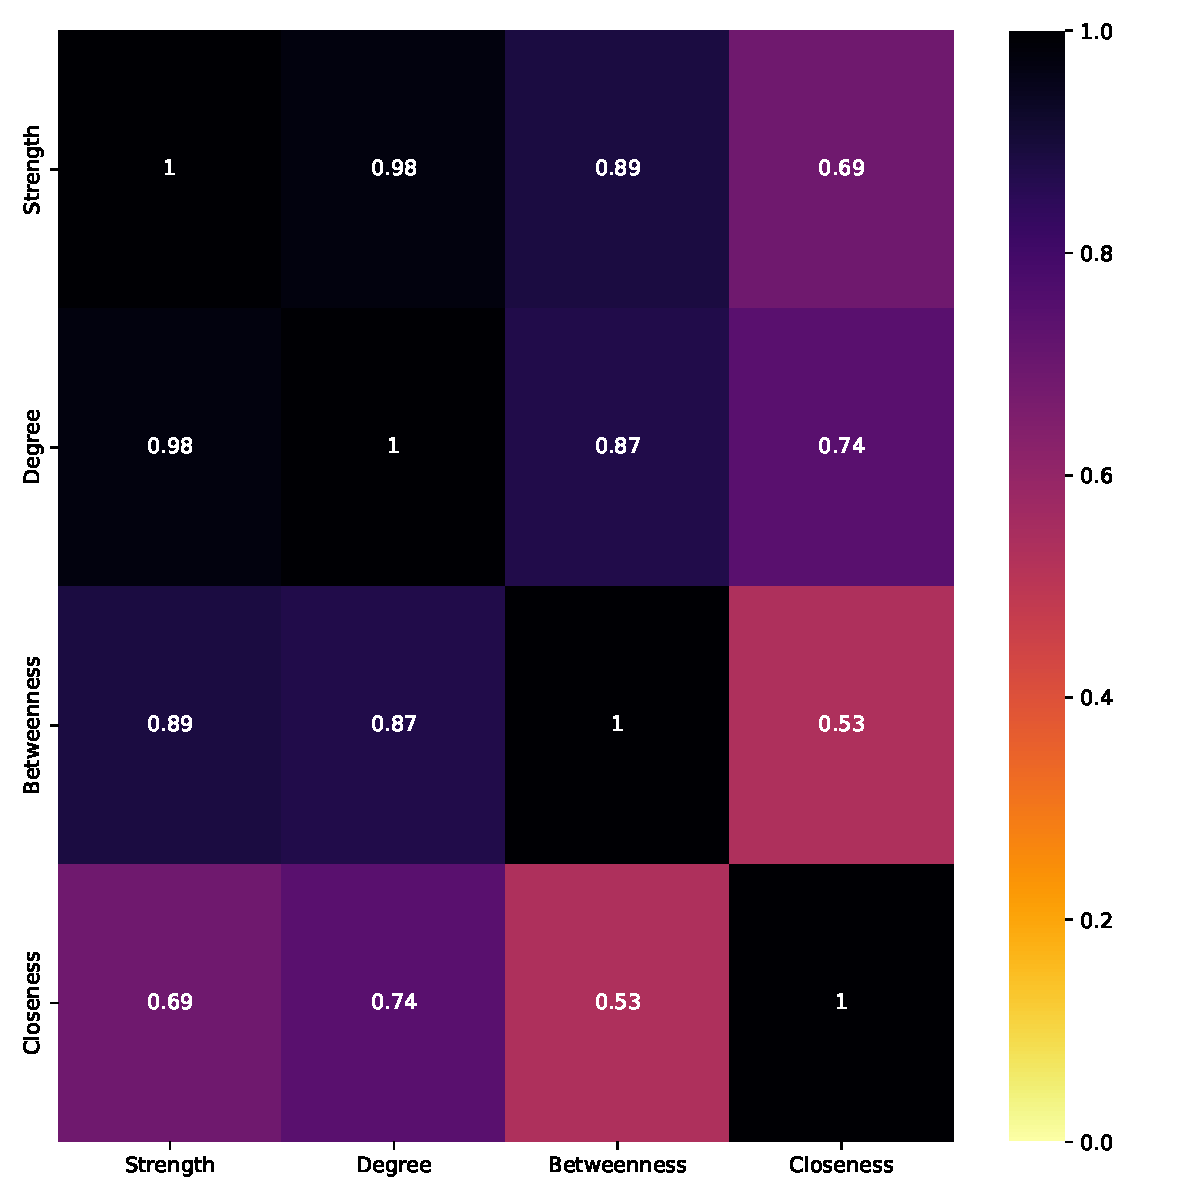
\includegraphics[scale=0.3]{companies/correlation_centrality.pdf}\\
 $=> $ Strength, degree and betweenness are highly correlated. Focus on strength as dependent variable.\\

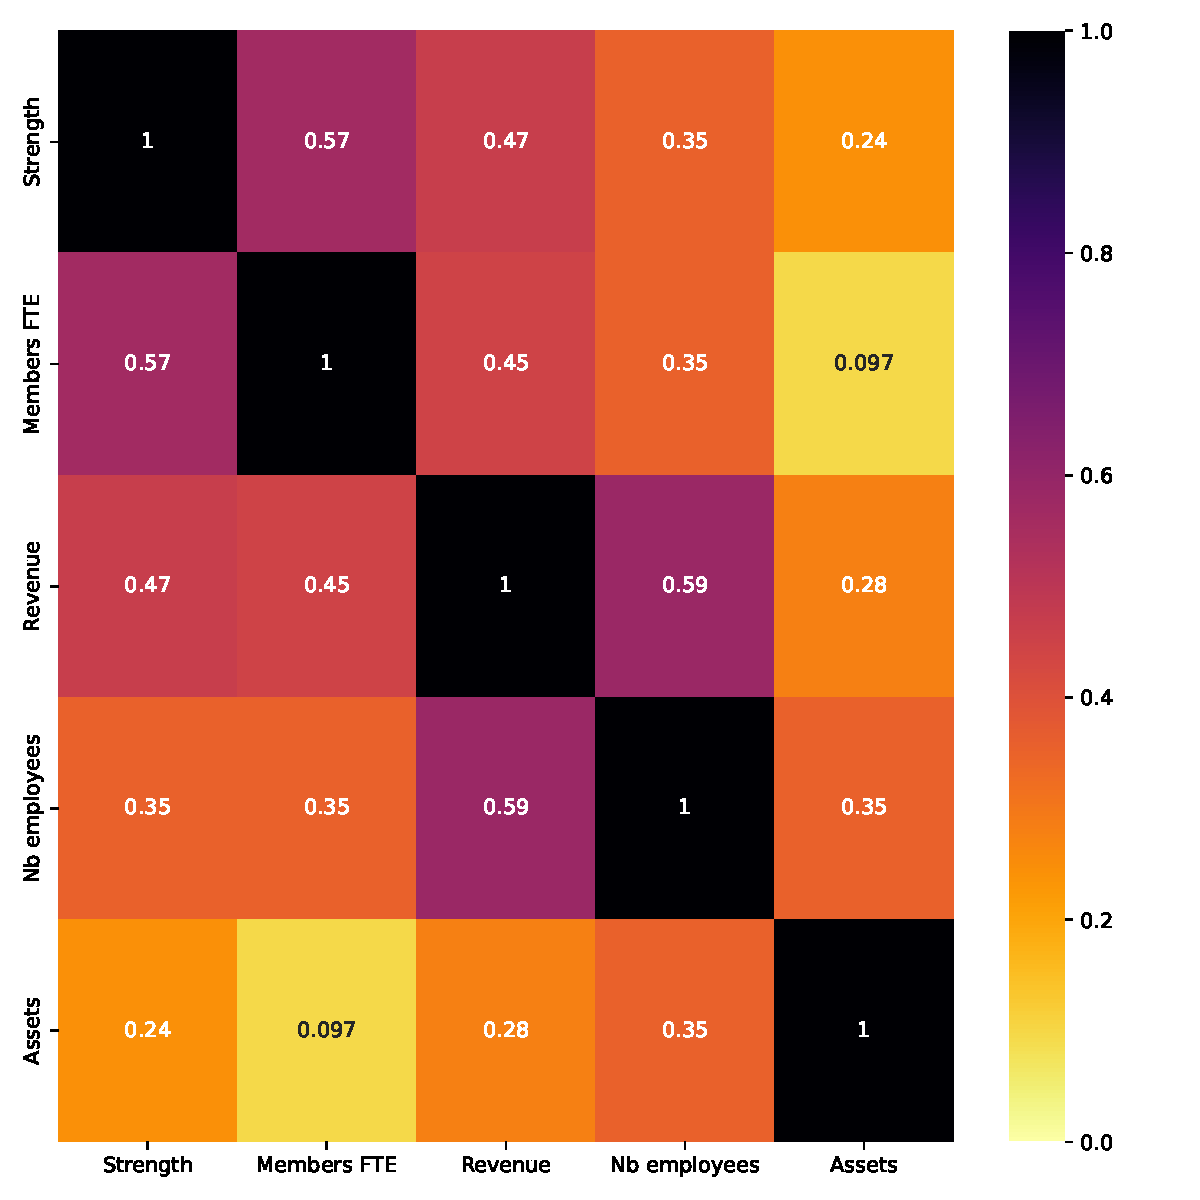
\includegraphics[scale=0.3]{companies/correlation_financials_lobbying_Strength.pdf}
\begin{itemize}
	\item Concerning financial data, revenue and number of employees are  highly correlated correlated. Surprisingly, the assets are weakly correlated to revenue and number of employees.
	\item Strength is highly correlated to Members FTE (expected). Relatively good correlation between Strength and Revenue.
\end{itemize}

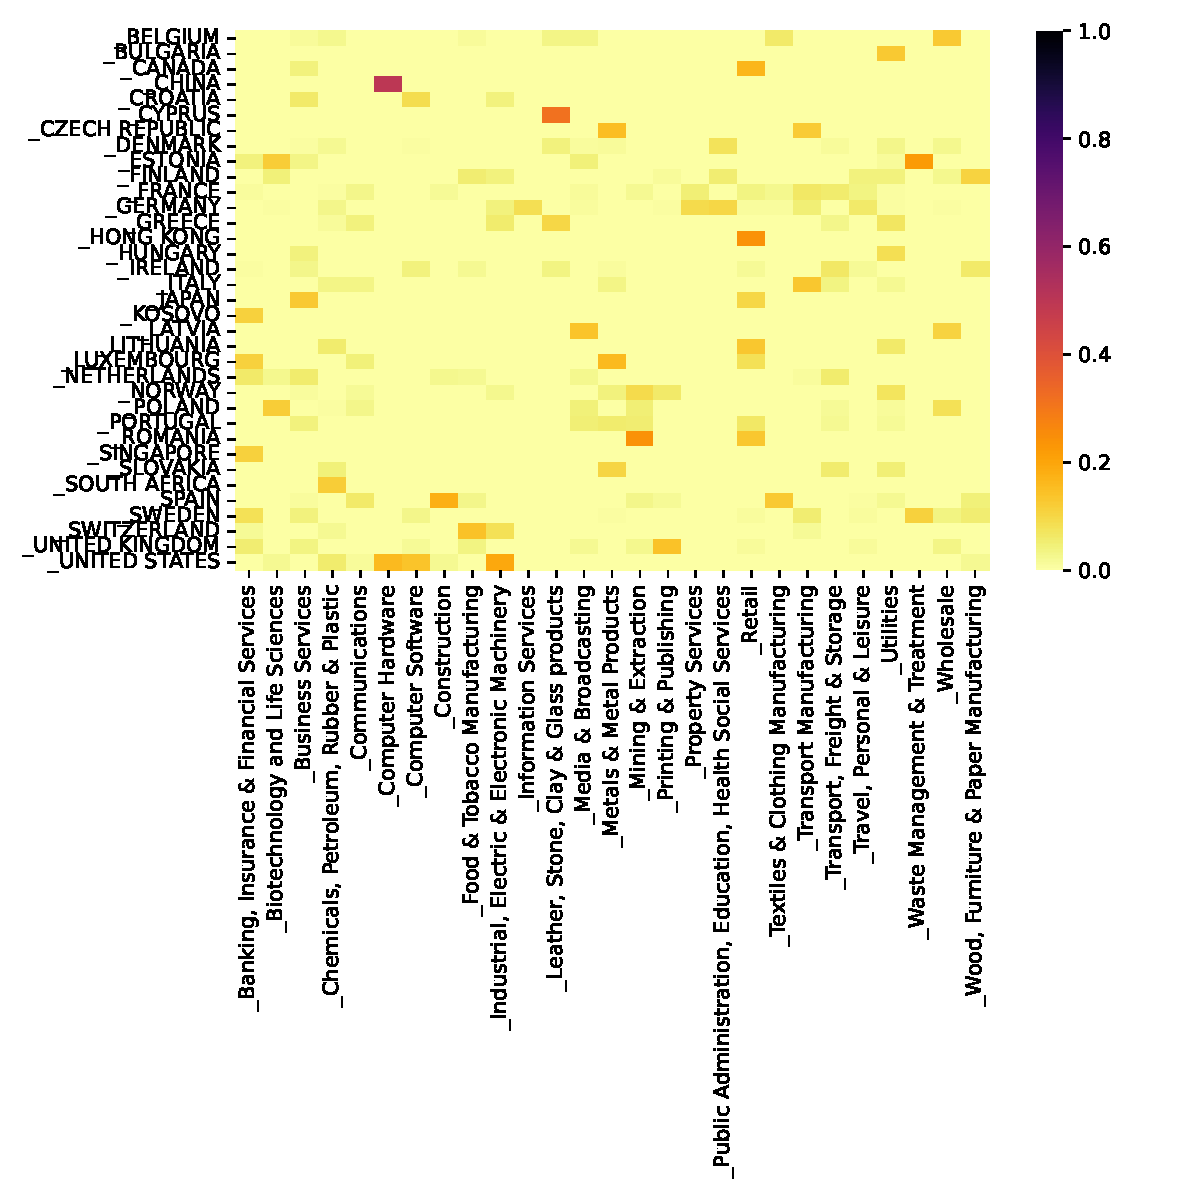
\includegraphics[scale=0.5]{companies/correlation_country_sector.pdf}
	\begin{itemize}
		\item High correlation between china and computer hardware. There is only one chinese company : Lenovo.  
		\item No other significant correlation.
	\end{itemize}

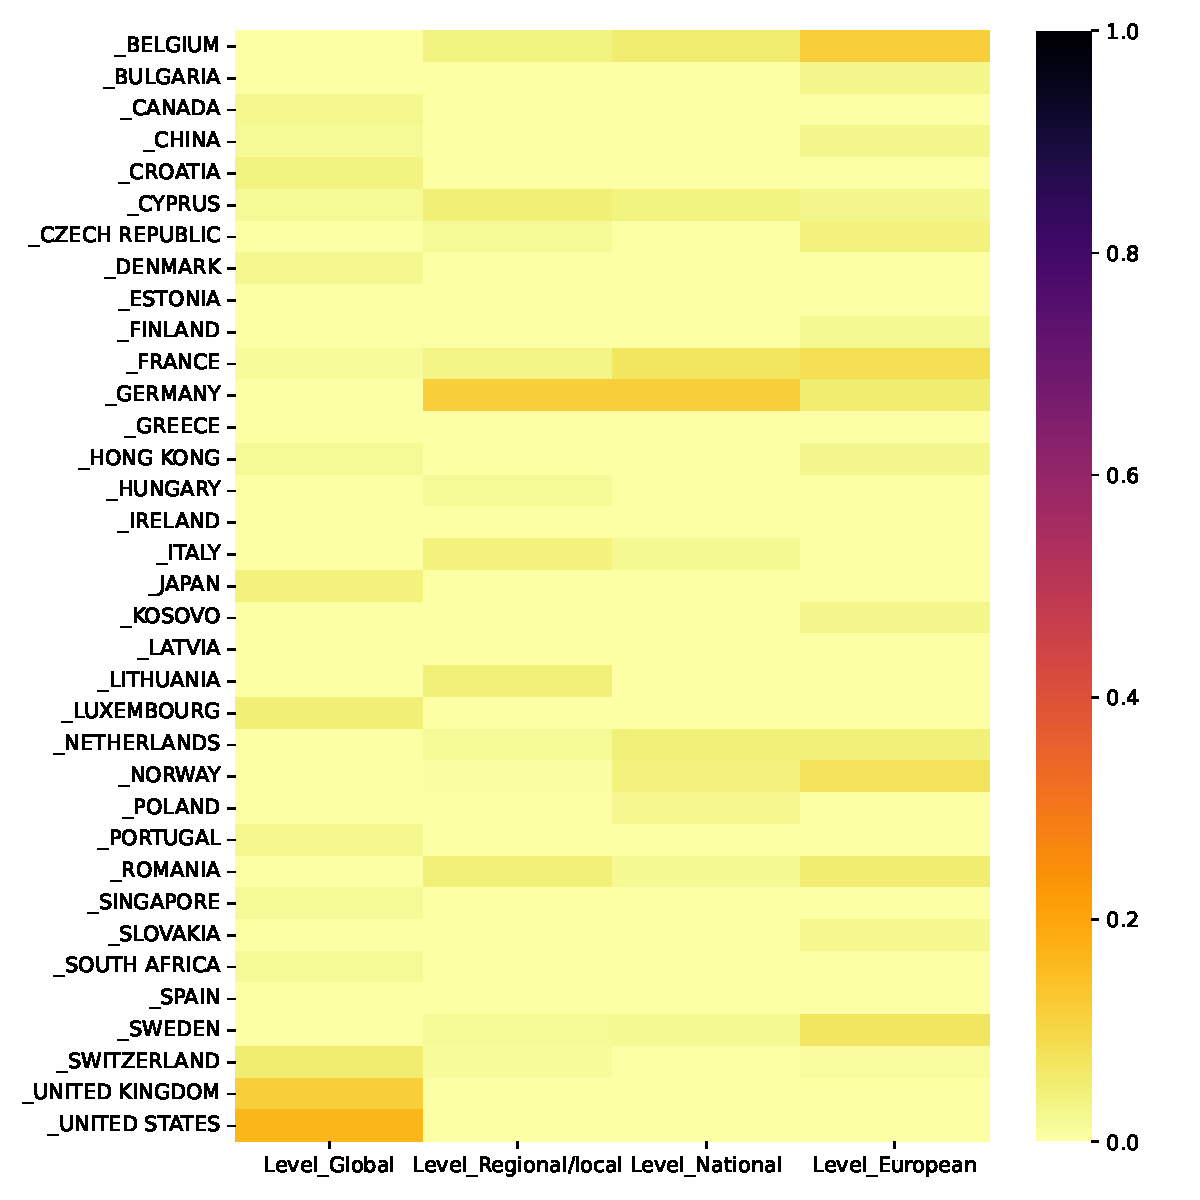
\includegraphics[scale=0.5]{companies/correlation_country_level.pdf}\\
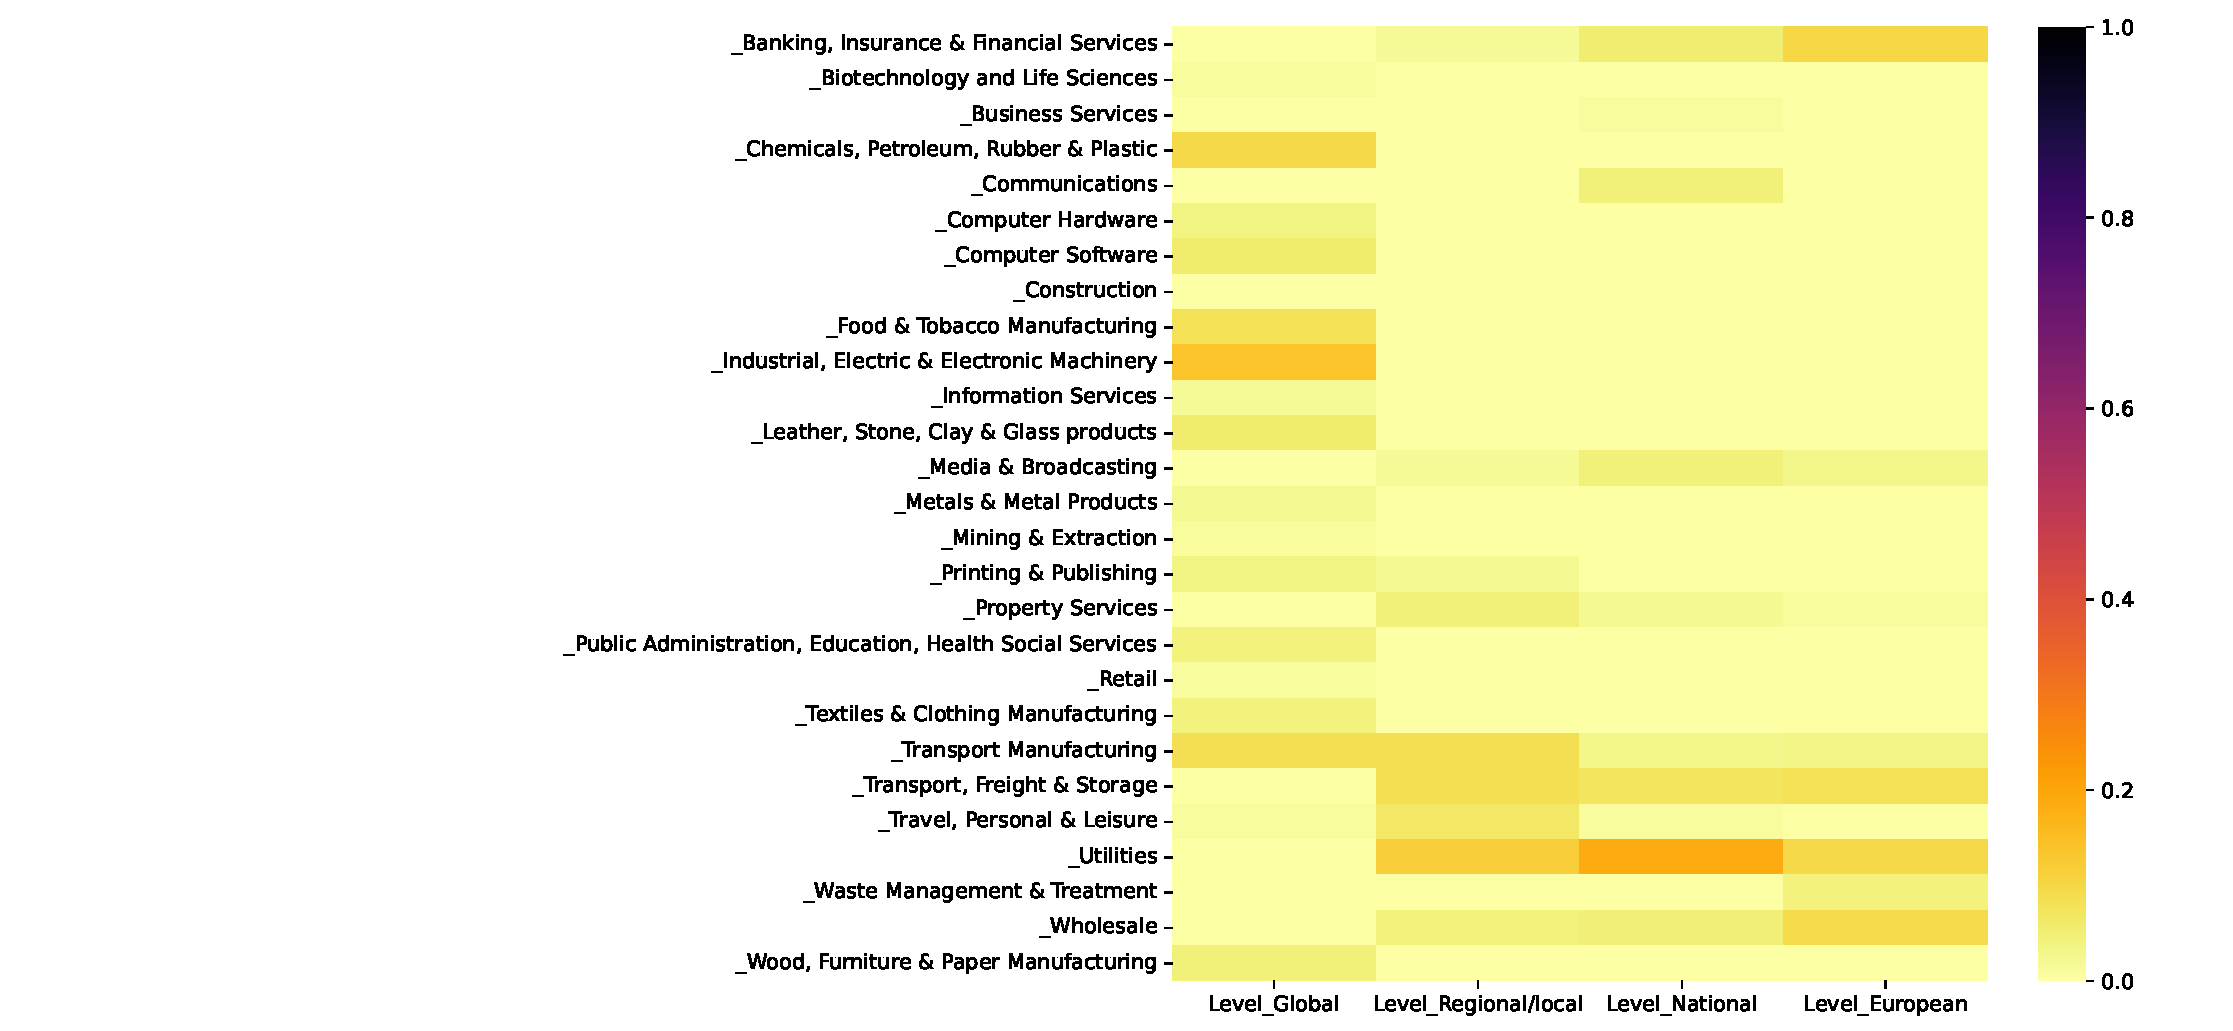
\includegraphics[scale=0.5]{companies/correlation_sector_level.pdf}

\begin{itemize}
	\item No significant relation.
	\end{itemize}
	
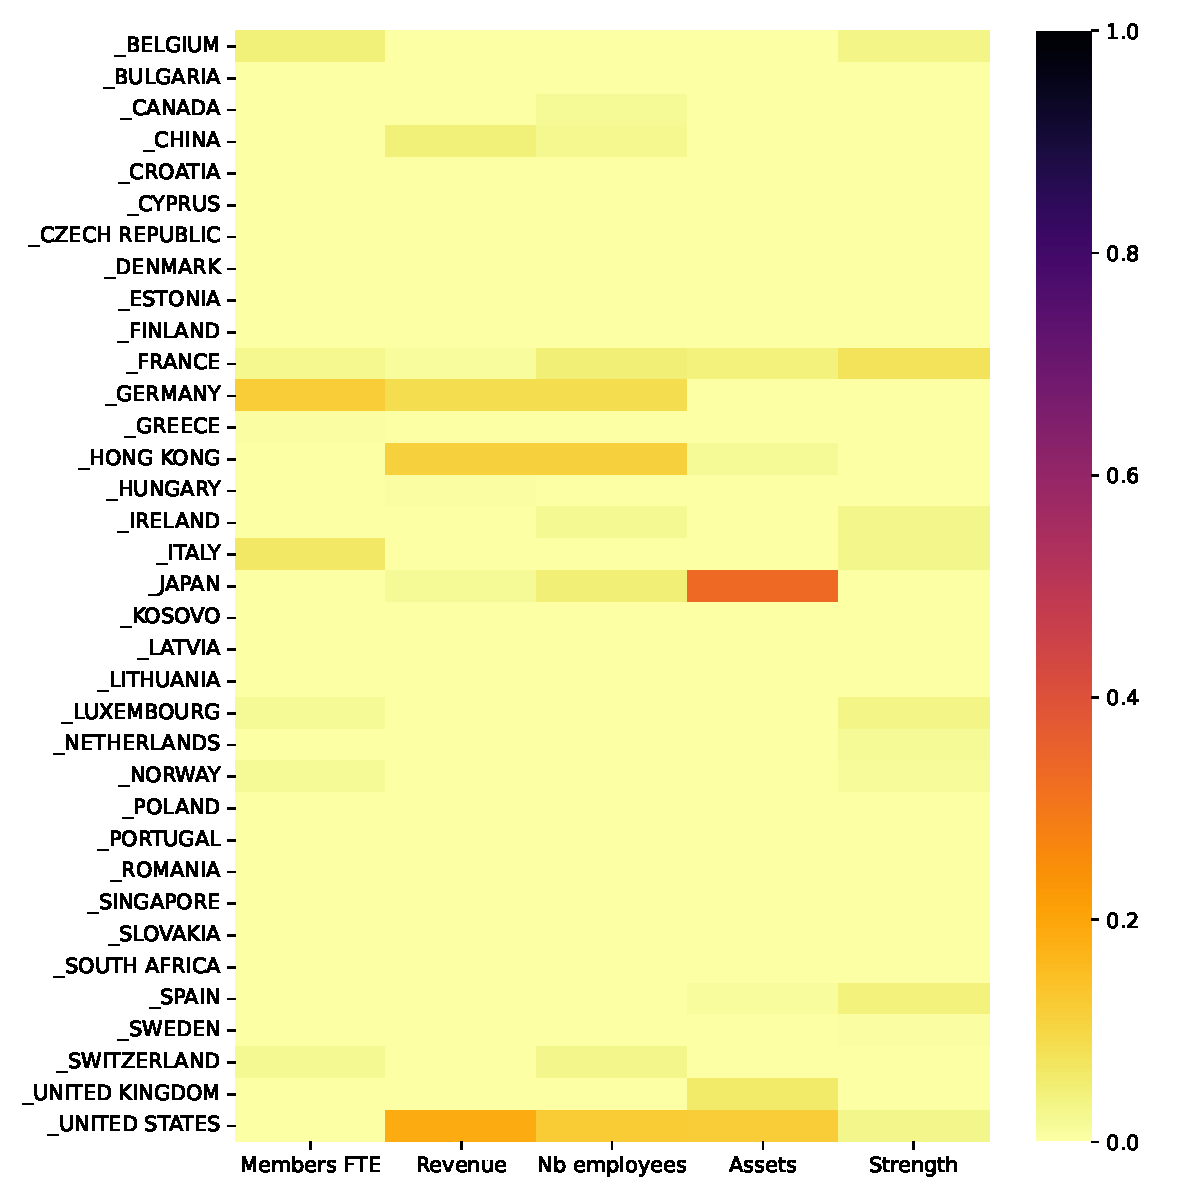
\includegraphics[scale=0.5]{companies/correlation_country_continuous.pdf}\\
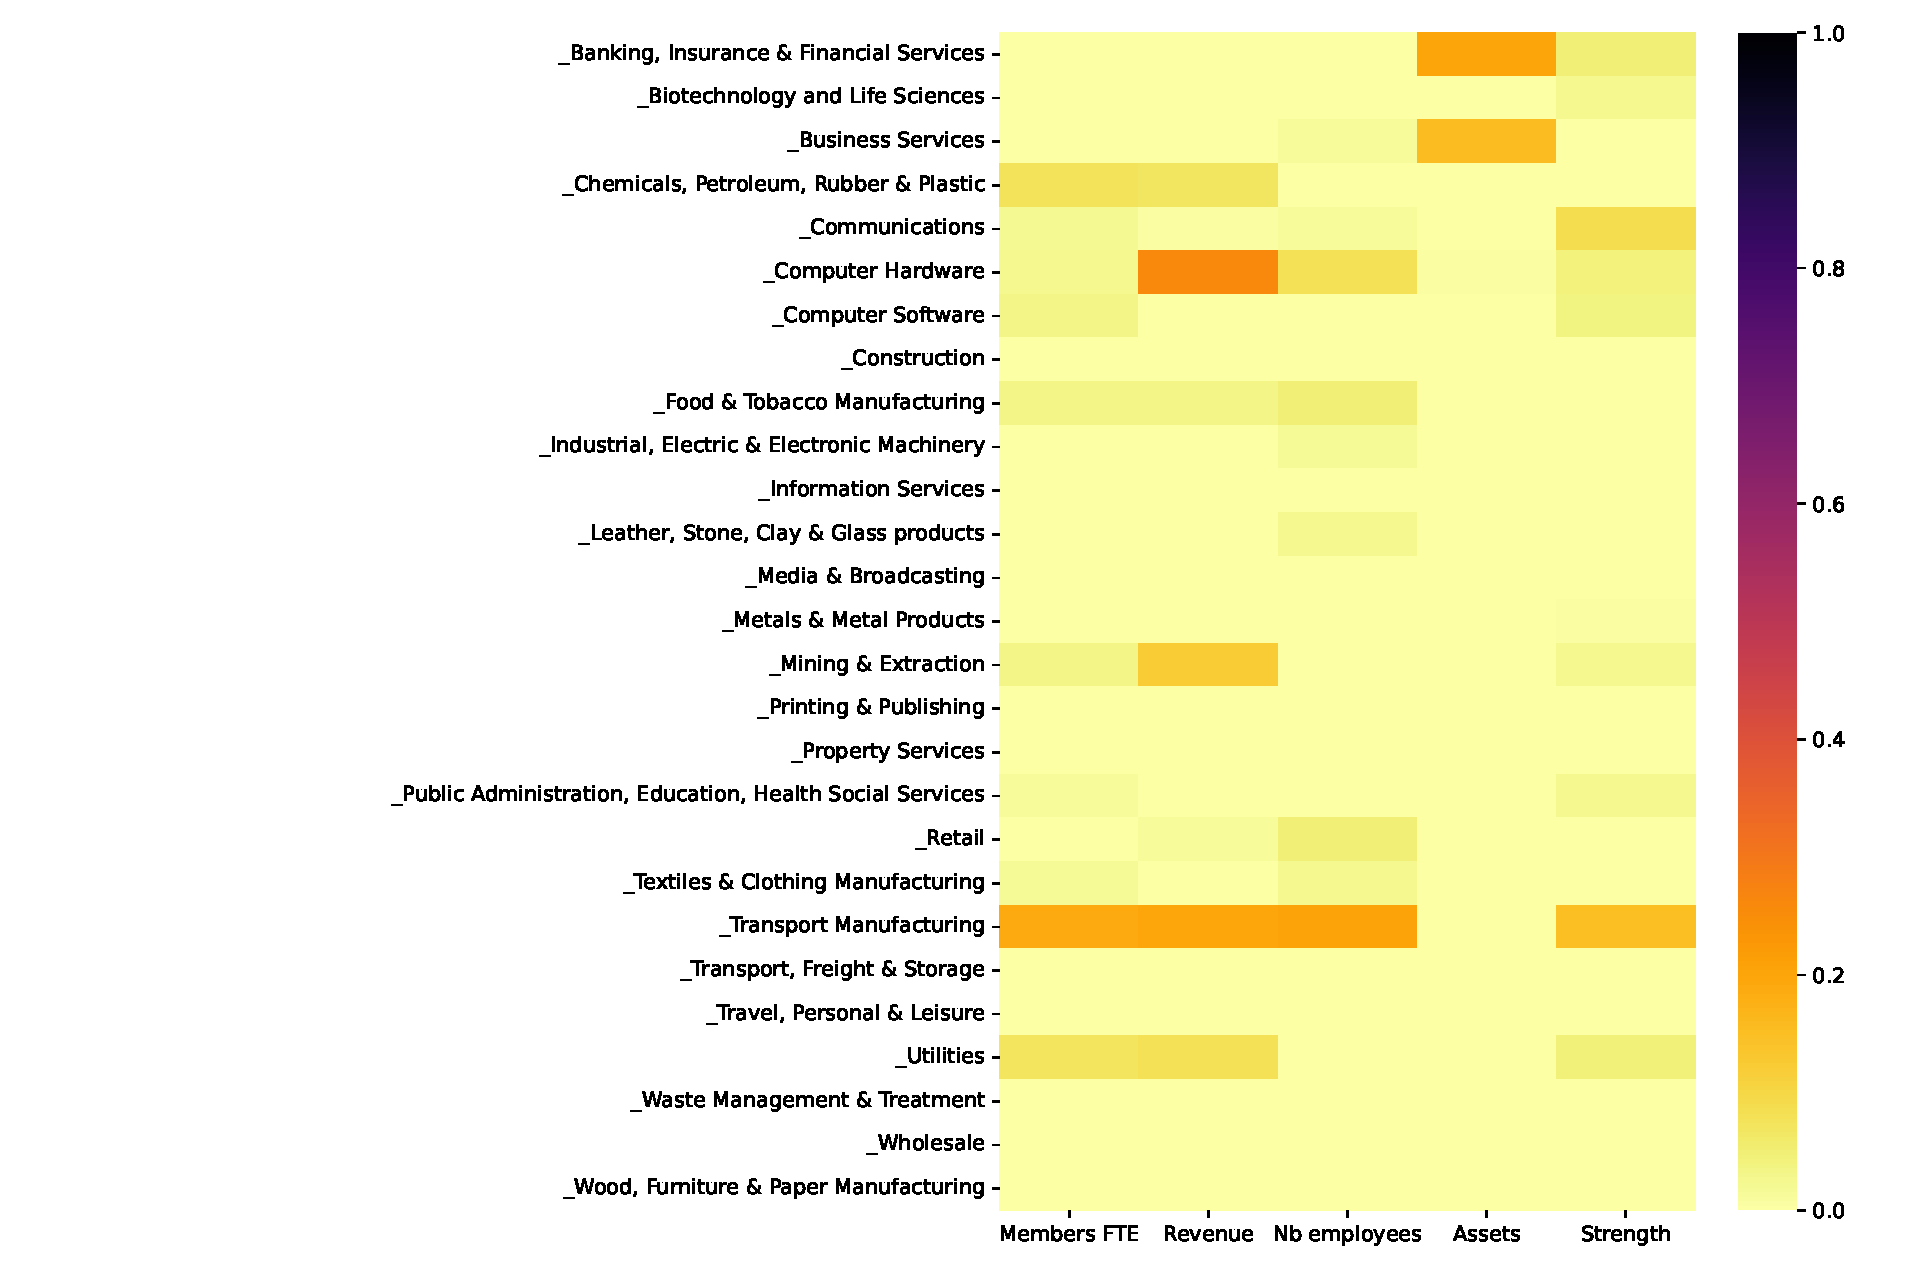
\includegraphics[scale=0.5]{companies/correlation_sector_continuous.pdf}\\
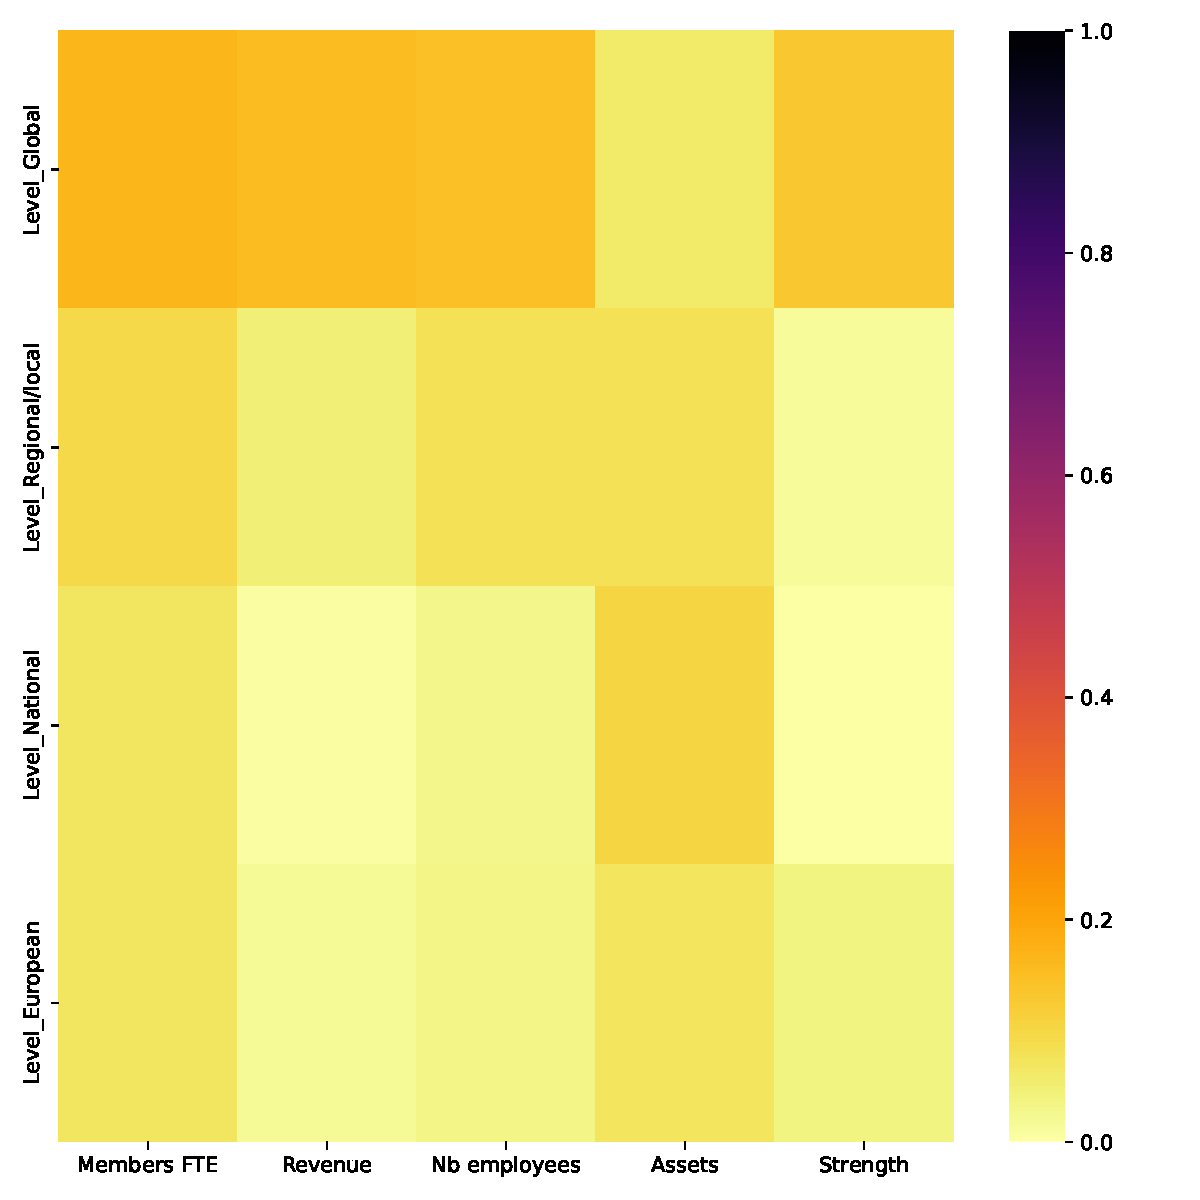
\includegraphics[scale=0.4]{companies/correlation_level_continuous.pdf}
	
	\subsection{Clean data}
	\subsubsection{Continuous}

\begin{tabular}{lr}
\toprule
 & Skew \\
\midrule
Assets & 6.833269 \\
Nb employees & 5.299134 \\
Revenue & 5.169145 \\
Strength & 4.095580 \\
Degree & 3.388787 \\
Members FTE & 3.032618 \\
Closeness & 0.495796 \\
Betweenness & 0.000000 \\
\bottomrule
\end{tabular}
	\begin{itemize}
		\item Numerical data are highly skewed.
		\item Closeness and Betweeneess seems to not be skewed. The plots shows that Betweenness is highly skewed. Should we normalize the centrality vector? This is surprising beacause, skeweness = $ \mathbb{E}[ (\frac{X-\mu}{\sigma})^3]$ \\
		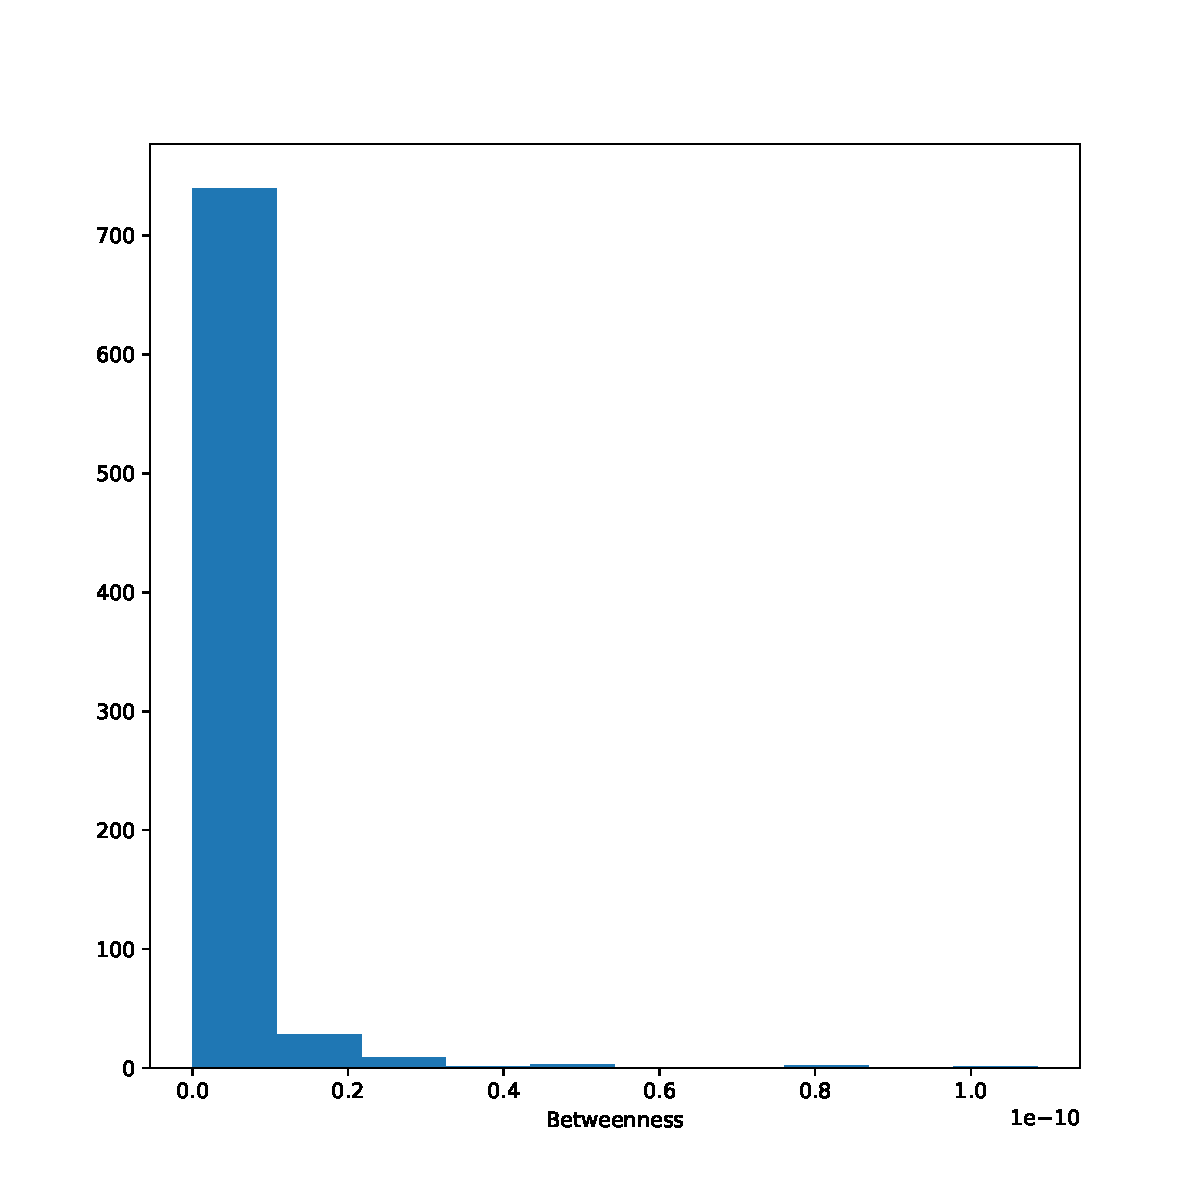
\includegraphics[scale=0.3]{companies/hist_btw.pdf} 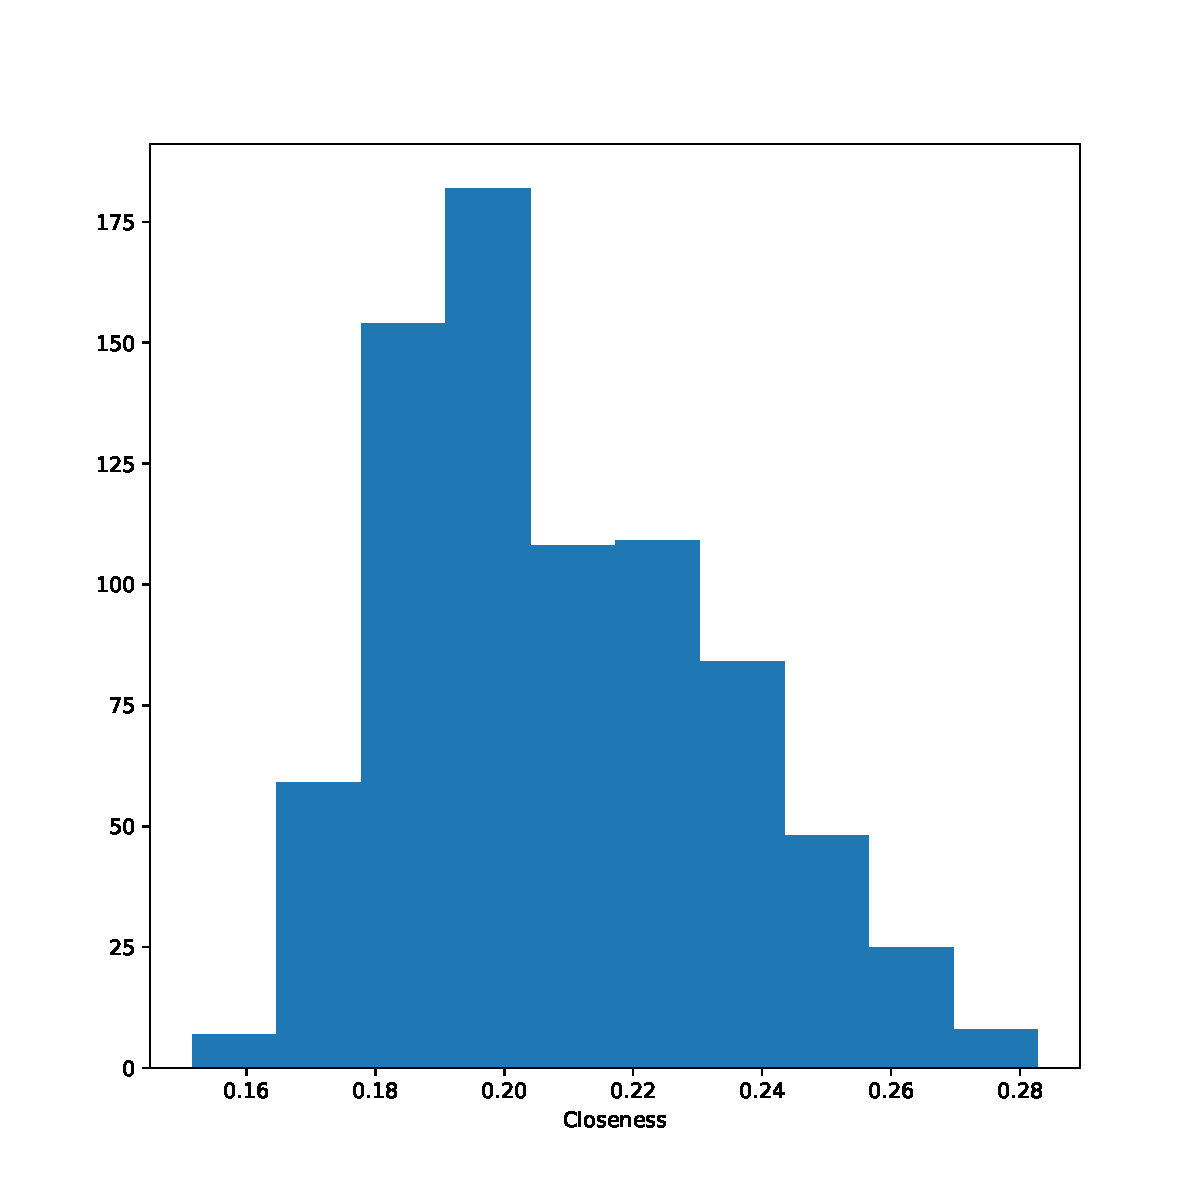
\includegraphics[scale=0.3]{companies/hist_cls.pdf}
		
	\item To handle skewness of variables, transform data. Use log transform and yeojohnson transform. To use log transform, we have to add 1 to all values to handle null values. And there is a company with negative revenue (Airholding S.A.). For the log transform, it has been removed. 
	\item log transform of independant variables. \\
	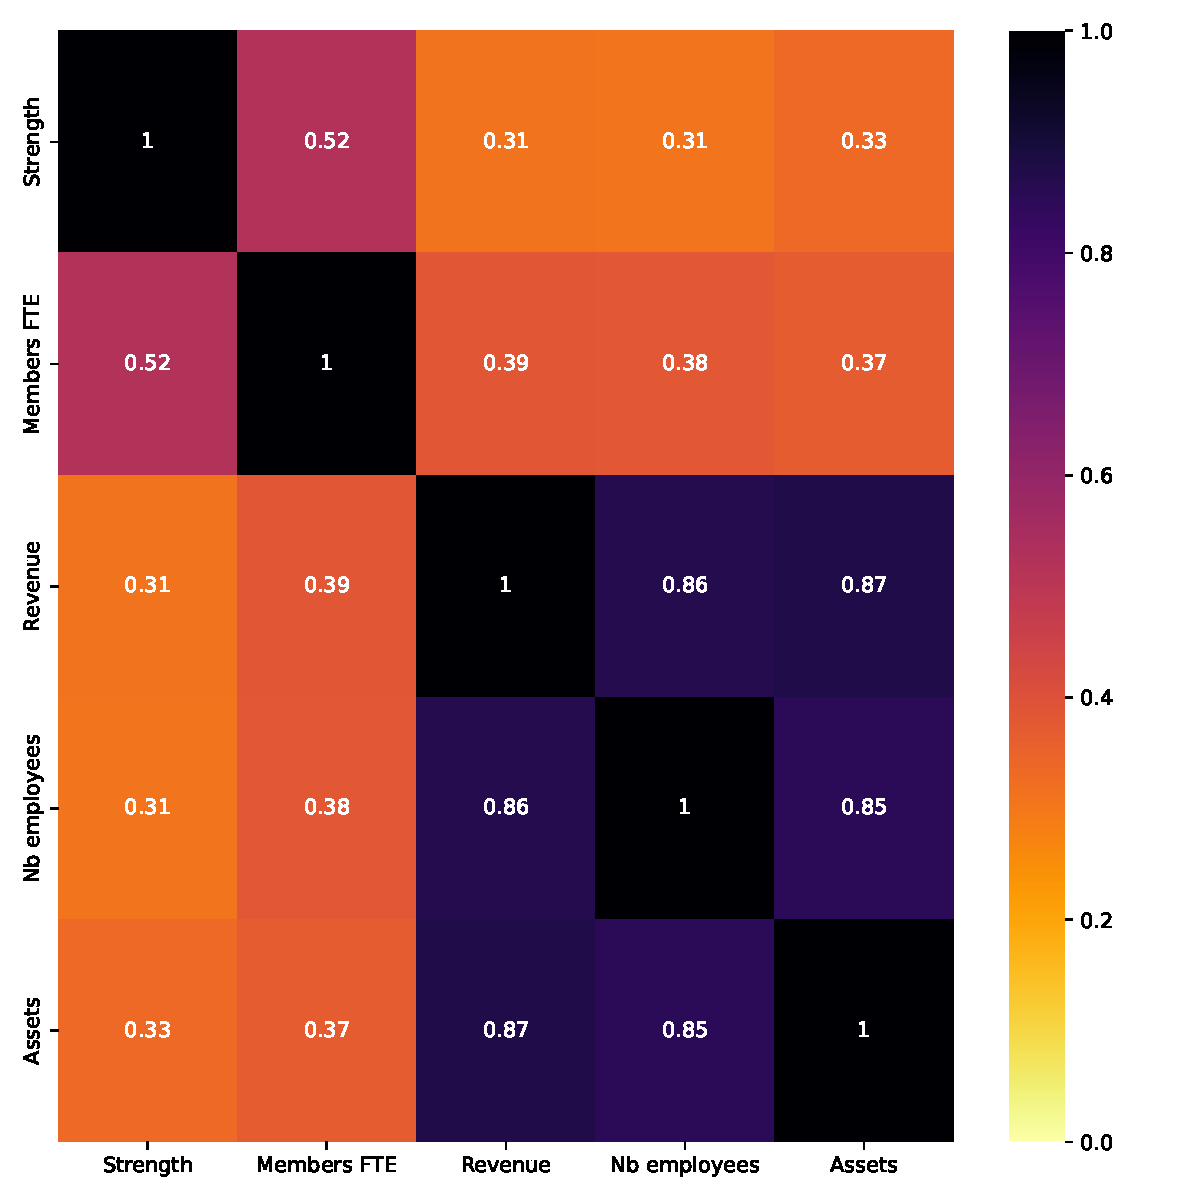
\includegraphics[scale=0.3]{companies/correlation_financials_lobbying_Strength_log.pdf}
	
	\item yeojohnson of independant variables\\
	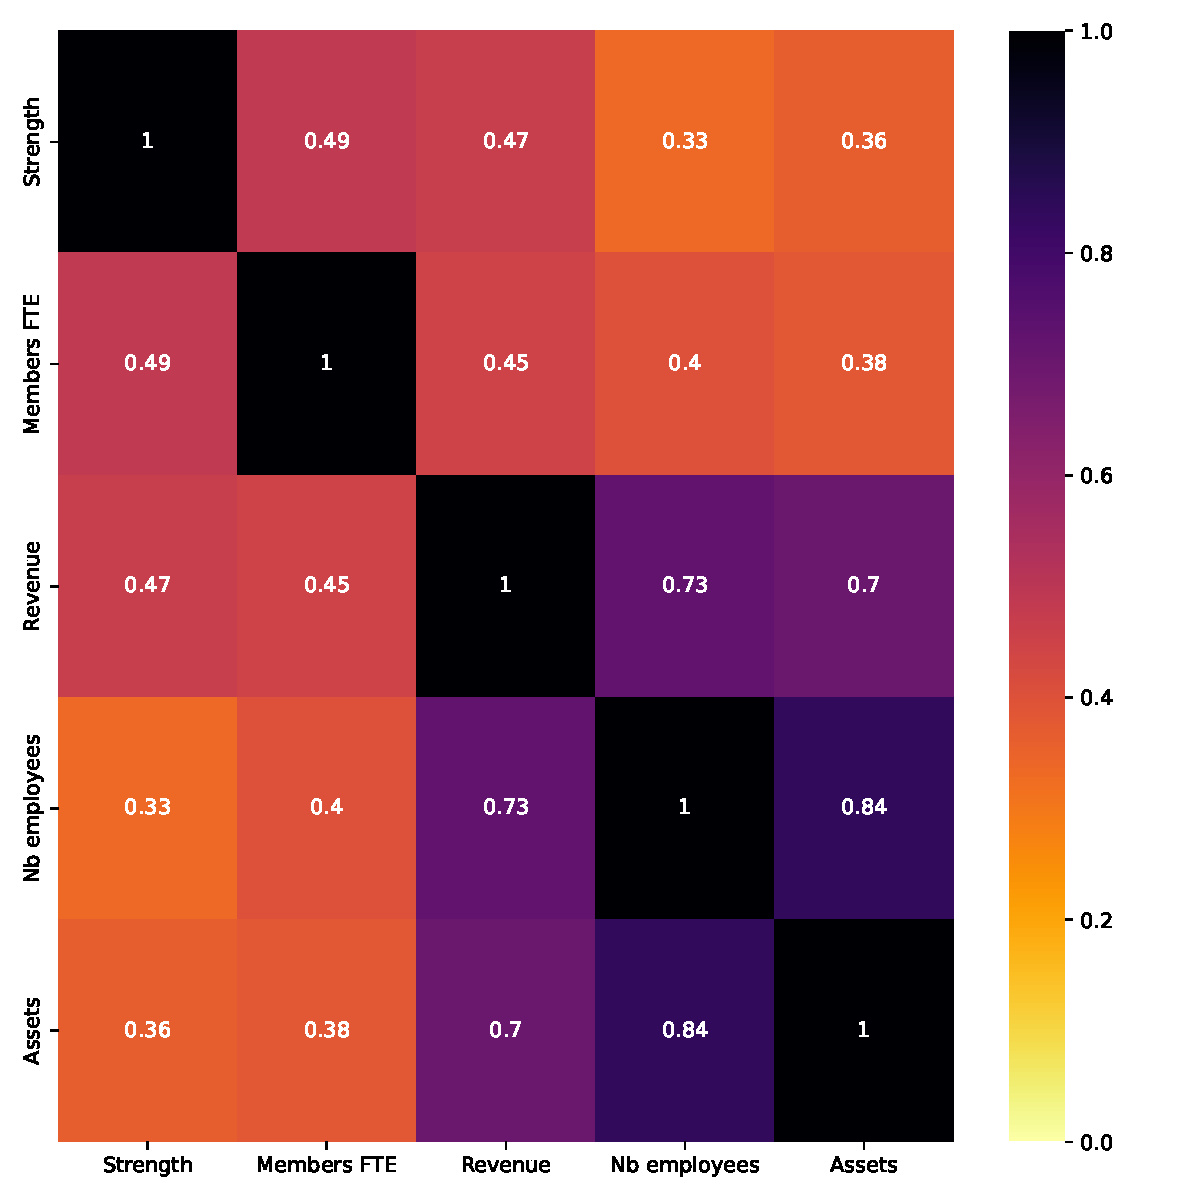
\includegraphics[scale=0.3]{companies/correlation_financials_lobbying_Strength_yeo.pdf}
	\item  Strengthen the correlation between financial data.
	\item Changes slightly the correlation between strength and the other variables. Except for assets which is considerably higher. The correlation between members FTE and assets also increases.
	\end{itemize}

	\subsubsection{Categorical}
	Categorical data are also highly skewed, in the sense that there are some categories that embed a low proportion of companies. Possible ways to overcome the problem: Remove outliers, or form fewer and larger categories, for instance group of countries. 
	
	\begin{itemize}
		\item Removing outliers: Define a frequency threshold under which the categories are considered to be very rare. All companies belonging to these categories are deleted. \\
		For thres =1\%,  \\removed category:  ['LUXEMBOURG', 'JAPAN', 'SLOVAKIA', 'CROATIA', 'ROMANIA', 'LITHUANIA', 'HUNGARY', 'CZECH REPUBLIC', 'CANADA', 'LATVIA', 'CYPRUS', 'CHINA', 'KOSOVO', 'SOUTH AFRICA', 'SINGAPORE', 'BULGARIA', 'HONG KONG']\\
number of outliers:  41\\
removed category:  ['Wood, Furniture and Paper Manufacturing', 'Biotechnology and Life Sciences', 'Construction', 'Public Administration, Education, Health Social Services', 'Textiles and Clothing Manufacturing', 'Agriculture, Horticulture and Livestock', 'Computer Hardware', 'Property Services', 'Waste Management and Treatment', 'Information Services']\\
number of outliers:  41
		\item Group country per region :     'North America': ['CANADA', 'UNITED STATES'],
    'North Europe': ['NORWAY', 'FINLAND', 'DENMARK', 'SWEDEN',  'LITHUANIA', 'LATVIA', 'ESTONIA', 'UNITED KINGDOM', 'IRELAND'],
    'South Europe': ['ITALY', 'SPAIN', 'PORTUGAL', 'GREECE', 'CROATIA', 'CYPRUS'],
    'East Europe': ['CZECH REPUBLIC', 'POLAND',   'ROMANIA', 'HUNGARY', 'BULGARIA', 'SLOVAKIA', 'KOSOVO'],
    'West Europe': ['AUSTRIA', 'GERMANY', 'SWITZERLAND', 'BELGIUM', 'LUXEMBOURG', 'FRANCE', 'NETHERLANDS'],
    'East Asia': ['JAPAN', 'CHINA', 'HONG KONG'],
    'Other': ['SOUTH AFRICA', 'SINGAPORE']
    \\ and remove outliers:
    removed category:  ['East Asia', 'Other']
number of outliers:  9\\
removed category:  ['Construction', 'Biotechnology and Life Sciences', 'Wood, Furniture and Paper Manufacturing', 'Textiles and Clothing Manufacturing', 'Public Administration, Education, Health Social Services', 'Agriculture, Horticulture and Livestock', 'Computer Hardware', 'Property Services', 'Waste Management and Treatment', 'Information Services']\\
number of outliers:  41
		
	\end{itemize}
	
	\newpage
	\subsection{Regression}
	\begin{center}
\begin{tabular}{lclc}
\toprule
\textbf{Dep. Variable:}    &      Strength      & \textbf{  R-squared:         } &     0.287   \\
\textbf{Model:}            &        OLS         & \textbf{  Adj. R-squared:    } &     0.285   \\
\textbf{Method:}           &   Least Squares    & \textbf{  F-statistic:       } &     140.7   \\
\textbf{Date:}             & jeu., 23 nov. 2023 & \textbf{  Prob (F-statistic):} &  4.61e-52   \\
\textbf{Time:}             &      11:27:28      & \textbf{  Log-Likelihood:    } &   -2582.7   \\
\textbf{No. Observations:} &          701       & \textbf{  AIC:               } &     5171.   \\
\textbf{Df Residuals:}     &          698       & \textbf{  BIC:               } &     5185.   \\
\textbf{Df Model:}         &            2       & \textbf{                     } &             \\
\textbf{Covariance Type:}  &     nonrobust      & \textbf{                     } &             \\
\bottomrule
\end{tabular}
\begin{tabular}{lcccccc}
                     & \textbf{coef} & \textbf{std err} & \textbf{t} & \textbf{P$> |$t$|$} & \textbf{[0.025} & \textbf{0.975]}  \\
\midrule
\textbf{const}       &      -7.2380  &        1.741     &    -4.157  &         0.000        &      -10.657    &       -3.819     \\
\textbf{Members FTE} &       9.1169  &        0.673     &    13.550  &         0.000        &        7.796    &       10.438     \\
\textbf{Revenue}     &       0.4766  &        0.129     &     3.704  &         0.000        &        0.224    &        0.729     \\
\bottomrule
\end{tabular}
\begin{tabular}{lclc}
\textbf{Omnibus:}       & 617.203 & \textbf{  Durbin-Watson:     } &     2.019  \\
\textbf{Prob(Omnibus):} &   0.000 & \textbf{  Jarque-Bera (JB):  } & 22252.246  \\
\textbf{Skew:}          &   3.801 & \textbf{  Prob(JB):          } &      0.00  \\
\textbf{Kurtosis:}      &  29.534 & \textbf{  Cond. No.          } &      70.6  \\
\bottomrule
\end{tabular}
%\caption{OLS Regression Results}
\end{center}

Notes: \newline
 [1] Standard Errors assume that the covariance matrix of the errors is correctly specified.

	\newpage
	\begin{center}
\begin{tabular}{lclc}
\toprule
\textbf{Dep. Variable:}    &      Strength      & \textbf{  R-squared:         } &     0.311   \\
\textbf{Model:}            &        OLS         & \textbf{  Adj. R-squared:    } &     0.290   \\
\textbf{Method:}           &   Least Squares    & \textbf{  F-statistic:       } &     15.32   \\
\textbf{Date:}             & jeu., 23 nov. 2023 & \textbf{  Prob (F-statistic):} &  6.51e-43   \\
\textbf{Time:}             &      11:28:13      & \textbf{  Log-Likelihood:    } &   -2571.0   \\
\textbf{No. Observations:} &          701       & \textbf{  AIC:               } &     5184.   \\
\textbf{Df Residuals:}     &          680       & \textbf{  BIC:               } &     5280.   \\
\textbf{Df Model:}         &           20       & \textbf{                     } &             \\
\textbf{Covariance Type:}  &     nonrobust      & \textbf{                     } &             \\
\bottomrule
\end{tabular}
\begin{tabular}{lcccccc}
                        & \textbf{coef} & \textbf{std err} & \textbf{t} & \textbf{P$> |$t$|$} & \textbf{[0.025} & \textbf{0.975]}  \\
\midrule
\textbf{const}          &     -10.2761  &        2.933     &    -3.504  &         0.000        &      -16.035    &       -4.517     \\
\textbf{Members FTE}    &       9.2331  &        0.688     &    13.422  &         0.000        &        7.882    &       10.584     \\
\textbf{Revenue}        &       0.4996  &        0.136     &     3.668  &         0.000        &        0.232    &        0.767     \\
\textbf{BELGIUM}        &       2.8760  &        2.891     &     0.995  &         0.320        &       -2.801    &        8.553     \\
\textbf{DENMARK}        &       0.4822  &        3.025     &     0.159  &         0.873        &       -5.457    &        6.422     \\
\textbf{ESTONIA}        &       5.0852  &        4.393     &     1.158  &         0.247        &       -3.540    &       13.710     \\
\textbf{FINLAND}        &       2.3868  &        2.801     &     0.852  &         0.394        &       -3.113    &        7.887     \\
\textbf{FRANCE}         &       4.6145  &        2.582     &     1.787  &         0.074        &       -0.455    &        9.684     \\
\textbf{GERMANY}        &       1.2260  &        2.511     &     0.488  &         0.626        &       -3.705    &        6.157     \\
\textbf{GREECE}         &      -1.1554  &        4.134     &    -0.280  &         0.780        &       -9.272    &        6.961     \\
\textbf{IRELAND}        &       6.8335  &        2.984     &     2.290  &         0.022        &        0.975    &       12.692     \\
\textbf{ITALY}          &       2.0536  &        2.776     &     0.740  &         0.460        &       -3.398    &        7.505     \\
\textbf{NETHERLANDS}    &       2.6211  &        2.621     &     1.000  &         0.318        &       -2.526    &        7.768     \\
\textbf{NORWAY}         &       3.2760  &        3.477     &     0.942  &         0.346        &       -3.550    &       10.102     \\
\textbf{POLAND}         &      -0.8174  &        3.966     &    -0.206  &         0.837        &       -8.605    &        6.970     \\
\textbf{PORTUGAL}       &       1.8545  &        4.133     &     0.449  &         0.654        &       -6.261    &        9.970     \\
\textbf{SPAIN}          &       5.5172  &        2.845     &     1.940  &         0.053        &       -0.068    &       11.102     \\
\textbf{SWEDEN}         &       4.5191  &        2.875     &     1.572  &         0.116        &       -1.125    &       10.163     \\
\textbf{SWITZERLAND}    &       0.8798  &        3.354     &     0.262  &         0.793        &       -5.705    &        7.465     \\
\textbf{UNITED KINGDOM} &       1.1134  &        2.600     &     0.428  &         0.669        &       -3.992    &        6.219     \\
\textbf{UNITED STATES}  &       2.7759  &        2.617     &     1.061  &         0.289        &       -2.363    &        7.915     \\
\bottomrule
\end{tabular}
\begin{tabular}{lclc}
\textbf{Omnibus:}       & 615.500 & \textbf{  Durbin-Watson:     } &     2.040  \\
\textbf{Prob(Omnibus):} &   0.000 & \textbf{  Jarque-Bera (JB):  } & 22797.653  \\
\textbf{Skew:}          &   3.771 & \textbf{  Prob(JB):          } &      0.00  \\
\textbf{Kurtosis:}      &  29.900 & \textbf{  Cond. No.          } &      423.  \\
\bottomrule
\end{tabular}
%\caption{OLS Regression Results}
\end{center}

Notes: \newline
 [1] Standard Errors assume that the covariance matrix of the errors is correctly specified.

\newpage
\begin{center}
\begin{tabular}{lclc}
\toprule
\textbf{Dep. Variable:}        &      Strength      & \textbf{  R-squared:         } &     0.318   \\
\textbf{Model:}                &        OLS         & \textbf{  Adj. R-squared:    } &     0.294   \\
\textbf{Method:}               &   Least Squares    & \textbf{  F-statistic:       } &     13.16   \\
\textbf{Date:}                 & jeu., 23 nov. 2023 & \textbf{  Prob (F-statistic):} &  3.82e-42   \\
\textbf{Time:}                 &      11:28:53      & \textbf{  Log-Likelihood:    } &   -2567.0   \\
\textbf{No. Observations:}     &          701       & \textbf{  AIC:               } &     5184.   \\
\textbf{Df Residuals:}         &          676       & \textbf{  BIC:               } &     5298.   \\
\textbf{Df Model:}             &           24       & \textbf{                     } &             \\
\textbf{Covariance Type:}      &     nonrobust      & \textbf{                     } &             \\
\bottomrule
\end{tabular}
\begin{tabular}{lcccccc}
                               & \textbf{coef} & \textbf{std err} & \textbf{t} & \textbf{P$> |$t$|$} & \textbf{[0.025} & \textbf{0.975]}  \\
\midrule
\textbf{const}                 &     -11.0216  &        3.015     &    -3.655  &         0.000        &      -16.942    &       -5.101     \\
\textbf{Members FTE}           &       9.0917  &        0.700     &    12.980  &         0.000        &        7.716    &       10.467     \\
\textbf{Revenue}               &       0.5220  &        0.137     &     3.818  &         0.000        &        0.254    &        0.790     \\
\textbf{BELGIUM}               &       2.6915  &        2.895     &     0.930  &         0.353        &       -2.993    &        8.376     \\
\textbf{DENMARK}               &       0.3113  &        3.025     &     0.103  &         0.918        &       -5.628    &        6.251     \\
\textbf{ESTONIA}               &       5.8645  &        4.402     &     1.332  &         0.183        &       -2.779    &       14.508     \\
\textbf{FINLAND}               &       2.2054  &        2.797     &     0.788  &         0.431        &       -3.287    &        7.698     \\
\textbf{FRANCE}                &       4.4594  &        2.584     &     1.726  &         0.085        &       -0.614    &        9.533     \\
\textbf{GERMANY}               &       1.3168  &        2.511     &     0.524  &         0.600        &       -3.614    &        6.248     \\
\textbf{GREECE}                &      -1.5470  &        4.127     &    -0.375  &         0.708        &       -9.651    &        6.557     \\
\textbf{IRELAND}               &       6.6049  &        2.980     &     2.216  &         0.027        &        0.753    &       12.457     \\
\textbf{ITALY}                 &       2.1511  &        2.770     &     0.777  &         0.438        &       -3.288    &        7.590     \\
\textbf{NETHERLANDS}           &       2.5494  &        2.620     &     0.973  &         0.331        &       -2.595    &        7.694     \\
\textbf{NORWAY}                &       3.0331  &        3.480     &     0.872  &         0.384        &       -3.800    &        9.866     \\
\textbf{POLAND}                &      -0.3867  &        3.964     &    -0.098  &         0.922        &       -8.170    &        7.397     \\
\textbf{PORTUGAL}              &       1.7514  &        4.137     &     0.423  &         0.672        &       -6.372    &        9.875     \\
\textbf{SPAIN}                 &       5.4544  &        2.840     &     1.921  &         0.055        &       -0.121    &       11.030     \\
\textbf{SWEDEN}                &       4.4722  &        2.871     &     1.558  &         0.120        &       -1.165    &       10.110     \\
\textbf{SWITZERLAND}           &       0.4808  &        3.356     &     0.143  &         0.886        &       -6.109    &        7.070     \\
\textbf{UNITED KINGDOM}        &       0.6191  &        2.613     &     0.237  &         0.813        &       -4.511    &        5.749     \\
\textbf{UNITED STATES}         &       2.1259  &        2.639     &     0.806  &         0.421        &       -3.055    &        7.307     \\
\textbf{Level\_Global}         &       1.3881  &        0.977     &     1.420  &         0.156        &       -0.531    &        3.307     \\
\textbf{Level\_Regional/local} &      -1.1356  &        1.049     &    -1.083  &         0.279        &       -3.195    &        0.924     \\
\textbf{Level\_National}       &      -1.4276  &        1.153     &    -1.238  &         0.216        &       -3.692    &        0.836     \\
\textbf{Level\_European}       &       1.2431  &        1.089     &     1.142  &         0.254        &       -0.894    &        3.380     \\
\bottomrule
\end{tabular}
\begin{tabular}{lclc}
\textbf{Omnibus:}       & 605.403 & \textbf{  Durbin-Watson:     } &     2.038  \\
\textbf{Prob(Omnibus):} &   0.000 & \textbf{  Jarque-Bera (JB):  } & 21348.090  \\
\textbf{Skew:}          &   3.692 & \textbf{  Prob(JB):          } &      0.00  \\
\textbf{Kurtosis:}      &  29.007 & \textbf{  Cond. No.          } &      425.  \\
\bottomrule
\end{tabular}
%\caption{OLS Regression Results}
\end{center}

Notes: \newline
 [1] Standard Errors assume that the covariance matrix of the errors is correctly specified.
 
 \newpage
 \begin{center}
\begin{tabular}{lclc}
\toprule
\textbf{Dep. Variable:}                                &      Strength      & \textbf{  R-squared:         } &     0.351   \\
\textbf{Model:}                                        &        OLS         & \textbf{  Adj. R-squared:    } &     0.311   \\
\textbf{Method:}                                       &   Least Squares    & \textbf{  F-statistic:       } &     8.699   \\
\textbf{Date:}                                         & jeu., 23 nov. 2023 & \textbf{  Prob (F-statistic):} &  8.16e-40   \\
\textbf{Time:}                                         &      11:29:55      & \textbf{  Log-Likelihood:    } &   -2549.8   \\
\textbf{No. Observations:}                             &          701       & \textbf{  AIC:               } &     5184.   \\
\textbf{Df Residuals:}                                 &          659       & \textbf{  BIC:               } &     5375.   \\
\textbf{Df Model:}                                     &           41       & \textbf{                     } &             \\
\textbf{Covariance Type:}                              &     nonrobust      & \textbf{                     } &             \\
\bottomrule
\end{tabular}
\begin{tabular}{lcccccc}
                                                       & \textbf{coef} & \textbf{std err} & \textbf{t} & \textbf{P$> |$t$|$} & \textbf{[0.025} & \textbf{0.975]}  \\
\midrule
\textbf{const}                                         &      -9.6483  &        3.326     &    -2.901  &         0.004        &      -16.179    &       -3.118     \\
\textbf{Members FTE}                                   &       8.7702  &        0.713     &    12.295  &         0.000        &        7.370    &       10.171     \\
\textbf{Revenue}                                       &       0.5868  &        0.143     &     4.092  &         0.000        &        0.305    &        0.868     \\
\textbf{BELGIUM}                                       &       3.2086  &        2.895     &     1.108  &         0.268        &       -2.477    &        8.894     \\
\textbf{DENMARK}                                       &       0.2917  &        3.012     &     0.097  &         0.923        &       -5.623    &        6.206     \\
\textbf{ESTONIA}                                       &       5.2046  &        4.390     &     1.186  &         0.236        &       -3.415    &       13.824     \\
\textbf{FINLAND}                                       &       1.9550  &        2.807     &     0.696  &         0.486        &       -3.557    &        7.467     \\
\textbf{FRANCE}                                        &       3.8888  &        2.600     &     1.496  &         0.135        &       -1.216    &        8.994     \\
\textbf{GERMANY}                                       &       1.0856  &        2.526     &     0.430  &         0.667        &       -3.874    &        6.045     \\
\textbf{GREECE}                                        &      -1.7418  &        4.108     &    -0.424  &         0.672        &       -9.808    &        6.324     \\
\textbf{IRELAND}                                       &       6.3297  &        2.990     &     2.117  &         0.035        &        0.459    &       12.200     \\
\textbf{ITALY}                                         &       1.6211  &        2.792     &     0.581  &         0.562        &       -3.861    &        7.103     \\
\textbf{NETHERLANDS}                                   &       2.0650  &        2.644     &     0.781  &         0.435        &       -3.126    &        7.256     \\
\textbf{NORWAY}                                        &       1.9121  &        3.477     &     0.550  &         0.583        &       -4.915    &        8.739     \\
\textbf{POLAND}                                        &      -0.2493  &        3.962     &    -0.063  &         0.950        &       -8.028    &        7.529     \\
\textbf{PORTUGAL}                                      &       1.8072  &        4.143     &     0.436  &         0.663        &       -6.327    &        9.941     \\
\textbf{SPAIN}                                         &       4.7100  &        2.850     &     1.653  &         0.099        &       -0.886    &       10.306     \\
\textbf{SWEDEN}                                        &       3.5027  &        2.892     &     1.211  &         0.226        &       -2.177    &        9.182     \\
\textbf{SWITZERLAND}                                   &       0.7414  &        3.381     &     0.219  &         0.826        &       -5.898    &        7.380     \\
\textbf{UNITED KINGDOM}                                &       0.1752  &        2.641     &     0.066  &         0.947        &       -5.011    &        5.361     \\
\textbf{UNITED STATES}                                 &       1.3205  &        2.669     &     0.495  &         0.621        &       -3.920    &        6.561     \\
\textbf{Level\_Global}                                 &       2.0791  &        1.013     &     2.052  &         0.041        &        0.089    &        4.069     \\
\textbf{Level\_Regional/local}                         &      -1.0351  &        1.049     &    -0.986  &         0.324        &       -3.096    &        1.026     \\
\textbf{Level\_National}                               &      -2.2249  &        1.172     &    -1.898  &         0.058        &       -4.526    &        0.076     \\
\textbf{Level\_European}                               &       1.5886  &        1.096     &     1.449  &         0.148        &       -0.564    &        3.741     \\
\textbf{Business Services}                             &      -1.4587  &        1.445     &    -1.010  &         0.313        &       -4.296    &        1.378     \\
\textbf{Chemicals, Petroleum, Rubber and Plastic}      &      -5.1945  &        1.713     &    -3.033  &         0.003        &       -8.558    &       -1.831     \\
\textbf{Communications}                                &       2.2225  &        2.029     &     1.095  &         0.274        &       -1.761    &        6.206     \\
\textbf{Computer Software}                             &      -0.1384  &        2.349     &    -0.059  &         0.953        &       -4.751    &        4.475     \\
\textbf{Food and Tobacco Manufacturing}                &      -6.2101  &        2.003     &    -3.101  &         0.002        &      -10.142    &       -2.278     \\
\textbf{Industrial, Electric and Electronic Machinery} &      -1.8404  &        1.700     &    -1.083  &         0.279        &       -5.178    &        1.497     \\
\textbf{Leather, Stone, Clay and Glass products}       &      -6.4808  &        3.476     &    -1.865  &         0.063        &      -13.305    &        0.344     \\
\textbf{Media and Broadcasting}                        &      -3.5353  &        2.324     &    -1.521  &         0.129        &       -8.098    &        1.028     \\
\textbf{Metals and Metal Products}                     &      -4.6243  &        2.683     &    -1.723  &         0.085        &       -9.893    &        0.644     \\
\textbf{Mining and Extraction}                         &      -2.1339  &        2.474     &    -0.863  &         0.389        &       -6.991    &        2.724     \\
\textbf{Printing and Publishing}                       &      -0.3381  &        3.038     &    -0.111  &         0.911        &       -6.303    &        5.627     \\
\textbf{Retail}                                        &      -2.1808  &        3.134     &    -0.696  &         0.487        &       -8.335    &        3.974     \\
\textbf{Transport Manufacturing}                       &       0.7652  &        2.177     &     0.351  &         0.725        &       -3.510    &        5.040     \\
\textbf{Transport, Freight and Storage}                &      -2.9440  &        1.835     &    -1.604  &         0.109        &       -6.547    &        0.659     \\
\textbf{Travel, Personal and Leisure}                  &      -2.3682  &        2.619     &    -0.904  &         0.366        &       -7.510    &        2.774     \\
\textbf{Utilities}                                     &      -0.3491  &        1.818     &    -0.192  &         0.848        &       -3.918    &        3.220     \\
\textbf{Wholesale}                                     &      -3.9676  &        1.973     &    -2.011  &         0.045        &       -7.841    &       -0.094     \\
\bottomrule
\end{tabular}
\begin{tabular}{lclc}
\textbf{Omnibus:}       & 597.253 & \textbf{  Durbin-Watson:     } &     2.053  \\
\textbf{Prob(Omnibus):} &   0.000 & \textbf{  Jarque-Bera (JB):  } & 20803.587  \\
\textbf{Skew:}          &   3.617 & \textbf{  Prob(JB):          } &      0.00  \\
\textbf{Kurtosis:}      &  28.689 & \textbf{  Cond. No.          } &      432.  \\
\bottomrule
\end{tabular}
%\caption{OLS Regression Results}
\end{center}

Notes: \newline
 [1] Standard Errors assume that the covariance matrix of the errors is correctly specified.
 
 
  \newpage
  \begin{center}
\begin{tabular}{lclc}
\toprule
\textbf{Dep. Variable:}                                    &      Strength      & \textbf{  R-squared:         } &     0.429   \\
\textbf{Model:}                                            &        OLS         & \textbf{  Adj. R-squared:    } &     0.353   \\
\textbf{Method:}                                           &   Least Squares    & \textbf{  F-statistic:       } &     5.654   \\
\textbf{Date:}                                             & jeu., 23 nov. 2023 & \textbf{  Prob (F-statistic):} &  1.11e-37   \\
\textbf{Time:}                                             &      11:30:54      & \textbf{  Log-Likelihood:    } &   -2505.2   \\
\textbf{No. Observations:}                                 &          701       & \textbf{  AIC:               } &     5176.   \\
\textbf{Df Residuals:}                                     &          618       & \textbf{  BIC:               } &     5554.   \\
\textbf{Df Model:}                                         &           82       & \textbf{                     } &             \\
\textbf{Covariance Type:}                                  &     nonrobust      & \textbf{                     } &             \\
\bottomrule
\end{tabular}
\begin{longtable}{lcccccc}
                                                           & \textbf{coef} & \textbf{std err} & \textbf{t} & \textbf{P$> |$t$|$} & \textbf{[0.025} & \textbf{0.975]}  \\
\midrule
\textbf{const}                                             &      -7.1791  &        3.445     &    -2.084  &         0.038        &      -13.945    &       -0.414     \\
\textbf{Members FTE}                                       &       7.7117  &        0.766     &    10.067  &         0.000        &        6.207    &        9.216     \\
\textbf{Revenue}                                           &       0.4816  &        0.153     &     3.141  &         0.002        &        0.181    &        0.783     \\
\textbf{BELGIUM}                                           &       1.3619  &        2.933     &     0.464  &         0.643        &       -4.397    &        7.121     \\
\textbf{DENMARK}                                           &      -0.3392  &        3.073     &    -0.110  &         0.912        &       -6.374    &        5.695     \\
\textbf{ESTONIA}                                           &       4.0585  &        4.408     &     0.921  &         0.358        &       -4.599    &       12.716     \\
\textbf{FINLAND}                                           &       0.5963  &        2.891     &     0.206  &         0.837        &       -5.080    &        6.273     \\
\textbf{FRANCE}                                            &       2.5189  &        2.692     &     0.936  &         0.350        &       -2.767    &        7.805     \\
\textbf{GERMANY}                                           &       0.3481  &        2.581     &     0.135  &         0.893        &       -4.720    &        5.416     \\
\textbf{GREECE}                                            &      -4.0497  &        4.113     &    -0.985  &         0.325        &      -12.127    &        4.027     \\
\textbf{IRELAND}                                           &       4.2560  &        3.038     &     1.401  &         0.162        &       -1.710    &       10.222     \\
\textbf{ITALY}                                             &       0.2485  &        2.822     &     0.088  &         0.930        &       -5.293    &        5.790     \\
\textbf{NETHERLANDS}                                       &       1.5577  &        2.672     &     0.583  &         0.560        &       -3.689    &        6.805     \\
\textbf{NORWAY}                                            &       1.6716  &        3.527     &     0.474  &         0.636        &       -5.254    &        8.597     \\
\textbf{POLAND}                                            &      -1.7669  &        3.966     &    -0.446  &         0.656        &       -9.555    &        6.022     \\
\textbf{PORTUGAL}                                          &      -1.1727  &        4.196     &    -0.279  &         0.780        &       -9.412    &        7.067     \\
\textbf{SPAIN}                                             &       3.0787  &        2.878     &     1.070  &         0.285        &       -2.574    &        8.731     \\
\textbf{SWEDEN}                                            &       2.4669  &        2.905     &     0.849  &         0.396        &       -3.238    &        8.172     \\
\textbf{SWITZERLAND}                                       &       0.3235  &        3.398     &     0.095  &         0.924        &       -6.349    &        6.996     \\
\textbf{UNITED KINGDOM}                                    &      -1.1348  &        2.677     &    -0.424  &         0.672        &       -6.392    &        4.122     \\
\textbf{UNITED STATES}                                     &      -0.6984  &        2.741     &    -0.255  &         0.799        &       -6.082    &        4.685     \\
\textbf{Level\_Global}                                     &       1.6715  &        1.024     &     1.632  &         0.103        &       -0.340    &        3.683     \\
\textbf{Level\_Regional/local}                             &      -1.0556  &        1.055     &    -1.001  &         0.317        &       -3.127    &        1.016     \\
\textbf{Level\_National}                                   &      -2.5848  &        1.190     &    -2.171  &         0.030        &       -4.923    &       -0.247     \\
\textbf{Level\_European}                                   &       1.7099  &        1.087     &     1.573  &         0.116        &       -0.424    &        3.844     \\
\textbf{Business Services}                                 &      -1.7561  &        1.642     &    -1.070  &         0.285        &       -4.980    &        1.468     \\
\textbf{Chemicals, Petroleum, Rubber and Plastic}          &      -3.3235  &        2.060     &    -1.613  &         0.107        &       -7.369    &        0.722     \\
\textbf{Communications}                                    &       1.0358  &        2.303     &     0.450  &         0.653        &       -3.487    &        5.558     \\
\textbf{Computer Software}                                 &      -0.4606  &        2.466     &    -0.187  &         0.852        &       -5.302    &        4.381     \\
\textbf{Food and Tobacco Manufacturing}                    &      -3.4284  &        2.543     &    -1.348  &         0.178        &       -8.422    &        1.565     \\
\textbf{Industrial, Electric and Electronic Machinery}     &      -2.1832  &        1.962     &    -1.113  &         0.266        &       -6.036    &        1.670     \\
\textbf{Leather, Stone, Clay and Glass products}           &      -7.2859  &        3.641     &    -2.001  &         0.046        &      -14.436    &       -0.135     \\
\textbf{Media and Broadcasting}                            &      -5.3056  &        2.632     &    -2.016  &         0.044        &      -10.474    &       -0.137     \\
\textbf{Metals and Metal Products}                         &      -4.9443  &        2.921     &    -1.692  &         0.091        &      -10.682    &        0.793     \\
\textbf{Mining and Extraction}                             &      -2.4928  &        2.669     &    -0.934  &         0.351        &       -7.735    &        2.749     \\
\textbf{Printing and Publishing}                           &      -0.5079  &        3.158     &    -0.161  &         0.872        &       -6.709    &        5.693     \\
\textbf{Retail}                                            &      -2.6218  &        3.216     &    -0.815  &         0.415        &       -8.937    &        3.693     \\
\textbf{Transport Manufacturing}                           &       1.0932  &        2.400     &     0.456  &         0.649        &       -3.619    &        5.805     \\
\textbf{Transport, Freight and Storage}                    &      -2.9095  &        2.184     &    -1.332  &         0.183        &       -7.199    &        1.380     \\
\textbf{Travel, Personal and Leisure}                      &      -2.6942  &        2.844     &    -0.947  &         0.344        &       -8.279    &        2.890     \\
\textbf{Utilities}                                         &      -0.2893  &        2.103     &    -0.138  &         0.891        &       -4.420    &        3.841     \\
\textbf{Wholesale}                                         &      -3.9665  &        2.233     &    -1.776  &         0.076        &       -8.352    &        0.419     \\
\textbf{Field\_Economy}                                    &      -1.5933  &        1.590     &    -1.002  &         0.317        &       -4.716    &        1.529     \\
\textbf{Field\_Enlargement}                                &      -0.7607  &        1.486     &    -0.512  &         0.609        &       -3.680    &        2.158     \\
\textbf{Field\_Food safety}                                &      -1.2572  &        1.374     &    -0.915  &         0.361        &       -3.956    &        1.442     \\
\textbf{Field\_Trans-European Networks}                    &      -1.7327  &        1.083     &    -1.600  &         0.110        &       -3.860    &        0.394     \\
\textbf{Field\_Business and industry}                      &      -0.1144  &        0.984     &    -0.116  &         0.908        &       -2.048    &        1.819     \\
\textbf{Field\_Agriculture and rural development}          &      -2.9188  &        2.417     &    -1.208  &         0.228        &       -7.665    &        1.827     \\
\textbf{Field\_Youth}                                      &       2.9097  &        1.730     &     1.681  &         0.093        &       -0.489    &        6.308     \\
\textbf{Field\_Migration and asylum}                       &       1.4437  &        2.790     &     0.517  &         0.605        &       -4.036    &        6.923     \\
\textbf{Field\_Climate action}                             &       1.5710  &        1.073     &     1.464  &         0.144        &       -0.536    &        3.678     \\
\textbf{Field\_Trade}                                      &       2.0820  &        0.977     &     2.130  &         0.034        &        0.163    &        4.001     \\
\textbf{Field\_Sport}                                      &      -5.8767  &        3.427     &    -1.715  &         0.087        &      -12.607    &        0.854     \\
\textbf{Field\_Borders and security}                       &       0.9023  &        1.384     &     0.652  &         0.515        &       -1.816    &        3.621     \\
\textbf{Field\_Culture and media}                          &       1.8925  &        2.209     &     0.857  &         0.392        &       -2.445    &        6.230     \\
\textbf{Field\_Humanitarian aid and civil protection}      &      -2.4737  &        1.802     &    -1.372  &         0.170        &       -6.013    &        1.066     \\
\textbf{Field\_Single market}                              &       0.9921  &        1.113     &     0.892  &         0.373        &       -1.193    &        3.177     \\
\textbf{Field\_finance and the euro}                       &      -0.1283  &        1.170     &    -0.110  &         0.913        &       -2.426    &        2.169     \\
\textbf{Field\_Education and training}                     &      -0.2808  &        1.183     &    -0.237  &         0.812        &       -2.604    &        2.043     \\
\textbf{Field\_Fraud prevention}                           &       0.7954  &        1.378     &     0.577  &         0.564        &       -1.912    &        3.502     \\
\textbf{Field\_Transport}                                  &       7.1557  &        3.461     &     2.067  &         0.039        &        0.359    &       13.953     \\
\textbf{Field\_Taxation}                                   &       0.6829  &        0.993     &     0.688  &         0.492        &       -1.267    &        2.633     \\
\textbf{Field\_Institutional affairs}                      &       1.1452  &        0.994     &     1.152  &         0.250        &       -0.807    &        3.097     \\
\textbf{Field\_International co-operation and development} &       1.5110  &        1.023     &     1.477  &         0.140        &       -0.498    &        3.520     \\
\textbf{Field\_Customs}                                    &      -2.8678  &        1.028     &    -2.789  &         0.005        &       -4.887    &       -0.849     \\
\textbf{Field\_External relations}                         &      -0.2037  &        1.034     &    -0.197  &         0.844        &       -2.234    &        1.827     \\
\textbf{Field\_Banking and financial services}             &      -0.7748  &        1.064     &    -0.728  &         0.467        &       -2.865    &        1.316     \\
\textbf{Field\_Maritime affairs and fisheries}             &      -1.4304  &        1.521     &    -0.940  &         0.347        &       -4.417    &        1.556     \\
\textbf{Field\_Competition}                                &      -0.3602  &        1.060     &    -0.340  &         0.734        &       -2.443    &        1.722     \\
\textbf{Field\_Energy}                                     &       1.1932  &        1.031     &     1.157  &         0.248        &       -0.832    &        3.218     \\
\textbf{Field\_Public health}                              &      -1.7018  &        1.129     &    -1.507  &         0.132        &       -3.920    &        0.516     \\
\textbf{Field\_Environment}                                &      -1.1906  &        1.152     &    -1.034  &         0.302        &       -3.452    &        1.071     \\
\textbf{Field\_Justice and fundamental rights}             &       2.4680  &        1.117     &     2.210  &         0.027        &        0.275    &        4.661     \\
\textbf{Field\_Culture}                                    &       1.6607  &        2.279     &     0.729  &         0.466        &       -2.815    &        6.136     \\
\textbf{Field\_Consumers}                                  &       0.8107  &        0.980     &     0.827  &         0.408        &       -1.114    &        2.735     \\
\textbf{Field\_Regional policy}                            &       0.5272  &        1.173     &     0.449  &         0.653        &       -1.777    &        2.831     \\
\textbf{Field\_Research and innovation}                    &      -1.1395  &        0.957     &    -1.191  &         0.234        &       -3.019    &        0.740     \\
\textbf{Field\_Digital economy and society}                &       0.5198  &        1.254     &     0.415  &         0.679        &       -1.942    &        2.982     \\
\textbf{Field\_Communication}                              &      -2.8663  &        1.153     &    -2.486  &         0.013        &       -5.131    &       -0.602     \\
\textbf{Field\_European neighbourhood policy}              &      -1.6818  &        1.974     &    -0.852  &         0.395        &       -5.559    &        2.196     \\
\textbf{Field\_Budget}                                     &       2.1216  &        1.198     &     1.771  &         0.077        &       -0.231    &        4.474     \\
\textbf{Field\_Employment and social affairs}              &       0.5258  &        0.997     &     0.527  &         0.598        &       -1.433    &        2.485     \\
\textbf{Field\_Foreign affairs and security policy}        &       0.2724  &        1.141     &     0.239  &         0.811        &       -1.968    &        2.513     \\
\bottomrule
\end{longtable}
\begin{tabular}{lclc}
\textbf{Omnibus:}       & 508.915 & \textbf{  Durbin-Watson:     } &     1.997  \\
\textbf{Prob(Omnibus):} &   0.000 & \textbf{  Jarque-Bera (JB):  } & 12246.707  \\
\textbf{Skew:}          &   2.950 & \textbf{  Prob(JB):          } &      0.00  \\
\textbf{Kurtosis:}      &  22.608 & \textbf{  Cond. No.          } &      461.  \\
\bottomrule
\end{tabular}
%\caption{OLS Regression Results}
\end{center}

Notes: \newline
 [1] Standard Errors assume that the covariance matrix of the errors is correctly specified.
 \newpage
 Group countries 

\begin{center}
\begin{tabular}{lclc}
\toprule
\textbf{Dep. Variable:}    &      Strength      & \textbf{  R-squared:         } &     0.291   \\
\textbf{Model:}            &        OLS         & \textbf{  Adj. R-squared:    } &     0.285   \\
\textbf{Method:}           &   Least Squares    & \textbf{  F-statistic:       } &     49.56   \\
\textbf{Date:}             & jeu., 23 nov. 2023 & \textbf{  Prob (F-statistic):} &  4.30e-51   \\
\textbf{Time:}             &      13:29:30      & \textbf{  Log-Likelihood:    } &   -2692.7   \\
\textbf{No. Observations:} &          733       & \textbf{  AIC:               } &     5399.   \\
\textbf{Df Residuals:}     &          726       & \textbf{  BIC:               } &     5432.   \\
\textbf{Df Model:}         &            6       & \textbf{                     } &             \\
\textbf{Covariance Type:}  &     nonrobust      & \textbf{                     } &             \\
\bottomrule
\end{tabular}
\begin{tabular}{lcccccc}
                      & \textbf{coef} & \textbf{std err} & \textbf{t} & \textbf{P$> |$t$|$} & \textbf{[0.025} & \textbf{0.975]}  \\
\midrule
\textbf{const}        &      -7.4138  &        2.199     &    -3.372  &         0.001        &      -11.731    &       -3.097     \\
\textbf{Members FTE}  &       8.9676  &        0.660     &    13.579  &         0.000        &        7.671    &       10.264     \\
\textbf{Revenue}      &       0.5054  &        0.126     &     3.996  &         0.000        &        0.257    &        0.754     \\
\textbf{East Europe}  &      -2.7490  &        2.345     &    -1.172  &         0.241        &       -7.353    &        1.855     \\
\textbf{North Europe} &       0.0925  &        1.329     &     0.070  &         0.945        &       -2.517    &        2.702     \\
\textbf{South Europe} &       0.2673  &        1.529     &     0.175  &         0.861        &       -2.734    &        3.268     \\
\textbf{West Europe}  &      -0.2286  &        1.273     &    -0.180  &         0.857        &       -2.727    &        2.270     \\
\bottomrule
\end{tabular}
\begin{tabular}{lclc}
\textbf{Omnibus:}       & 643.431 & \textbf{  Durbin-Watson:     } &     2.000  \\
\textbf{Prob(Omnibus):} &   0.000 & \textbf{  Jarque-Bera (JB):  } & 23420.226  \\
\textbf{Skew:}          &   3.794 & \textbf{  Prob(JB):          } &      0.00  \\
\textbf{Kurtosis:}      &  29.631 & \textbf{  Cond. No.          } &      130.  \\
\bottomrule
\end{tabular}
%\caption{OLS Regression Results}
\end{center}

Notes: \newline
 [1] Standard Errors assume that the covariance matrix of the errors is correctly specified.
 
\begin{center}

\begin{tabular}{lcccccc}
                       & \textbf{coef} & \textbf{std err} & \textbf{t} & \textbf{P$> |$t$|$} & \textbf{[0.025} & \textbf{0.975]}  \\
\midrule
\textbf{const}         &     -10.1629  &        2.625     &    -3.871  &         0.000        &      -15.317    &       -5.009     \\
\textbf{Members FTE}   &       8.9676  &        0.660     &    13.579  &         0.000        &        7.671    &       10.264     \\
\textbf{Revenue}       &       0.5054  &        0.126     &     3.996  &         0.000        &        0.257    &        0.754     \\
\textbf{North America} &       2.7490  &        2.345     &     1.172  &         0.241        &       -1.855    &        7.353     \\
\textbf{North Europe}  &       2.8415  &        2.142     &     1.327  &         0.185        &       -1.363    &        7.046     \\
\textbf{South Europe}  &       3.0164  &        2.267     &     1.330  &         0.184        &       -1.435    &        7.467     \\
\textbf{West Europe}   &       2.5204  &        2.115     &     1.192  &         0.234        &       -1.632    &        6.673     \\
\bottomrule
\end{tabular}
\begin{tabular}{lclc}
\textbf{Omnibus:}       & 643.431 & \textbf{  Durbin-Watson:     } &     2.000  \\
\textbf{Prob(Omnibus):} &   0.000 & \textbf{  Jarque-Bera (JB):  } & 23420.226  \\
\textbf{Skew:}          &   3.794 & \textbf{  Prob(JB):          } &      0.00  \\
\textbf{Kurtosis:}      &  29.631 & \textbf{  Cond. No.          } &      195.  \\
\bottomrule
\end{tabular}
%\caption{OLS Regression Results}
\end{center}

Notes: \newline
 [1] Standard Errors assume that the covariance matrix of the errors is correctly specified.
 \newpage
 \begin{center}
\begin{tabular}{lclc}
\toprule
\textbf{Dep. Variable:}        &      Strength      & \textbf{  R-squared:         } &     0.298   \\
\textbf{Model:}                &        OLS         & \textbf{  Adj. R-squared:    } &     0.289   \\
\textbf{Method:}               &   Least Squares    & \textbf{  F-statistic:       } &     30.71   \\
\textbf{Date:}                 & jeu., 23 nov. 2023 & \textbf{  Prob (F-statistic):} &  1.63e-49   \\
\textbf{Time:}                 &      13:32:30      & \textbf{  Log-Likelihood:    } &   -2688.7   \\
\textbf{No. Observations:}     &          733       & \textbf{  AIC:               } &     5399.   \\
\textbf{Df Residuals:}         &          722       & \textbf{  BIC:               } &     5450.   \\
\textbf{Df Model:}             &           10       & \textbf{                     } &             \\
\textbf{Covariance Type:}      &     nonrobust      & \textbf{                     } &             \\
\bottomrule
\end{tabular}
\begin{tabular}{lcccccc}
                               & \textbf{coef} & \textbf{std err} & \textbf{t} & \textbf{P$> |$t$|$} & \textbf{[0.025} & \textbf{0.975]}  \\
\midrule
\textbf{const}                 &     -10.6712  &        2.702     &    -3.949  &         0.000        &      -15.977    &       -5.365     \\
\textbf{Members FTE}           &       8.8800  &        0.672     &    13.220  &         0.000        &        7.561    &       10.199     \\
\textbf{Revenue}               &       0.5289  &        0.127     &     4.168  &         0.000        &        0.280    &        0.778     \\
\textbf{North America}         &       2.1840  &        2.423     &     0.901  &         0.368        &       -2.573    &        6.941     \\
\textbf{North Europe}          &       2.6081  &        2.175     &     1.199  &         0.231        &       -1.663    &        6.879     \\
\textbf{South Europe}          &       2.9697  &        2.295     &     1.294  &         0.196        &       -1.536    &        7.475     \\
\textbf{West Europe}           &       2.4348  &        2.146     &     1.134  &         0.257        &       -1.779    &        6.648     \\
\textbf{Level\_Global}         &       1.0013  &        0.926     &     1.081  &         0.280        &       -0.817    &        2.820     \\
\textbf{Level\_Regional/local} &      -1.1832  &        1.001     &    -1.182  &         0.238        &       -3.149    &        0.782     \\
\textbf{Level\_National}       &      -1.5859  &        1.106     &    -1.434  &         0.152        &       -3.756    &        0.585     \\
\textbf{Level\_European}       &       1.4246  &        1.029     &     1.384  &         0.167        &       -0.596    &        3.445     \\
\bottomrule
\end{tabular}
\begin{tabular}{lclc}
\textbf{Omnibus:}       & 632.414 & \textbf{  Durbin-Watson:     } &     2.003  \\
\textbf{Prob(Omnibus):} &   0.000 & \textbf{  Jarque-Bera (JB):  } & 21852.233  \\
\textbf{Skew:}          &   3.712 & \textbf{  Prob(JB):          } &      0.00  \\
\textbf{Kurtosis:}      &  28.698 & \textbf{  Cond. No.          } &      199.  \\
\bottomrule
\end{tabular}
%\caption{OLS Regression Results}
\end{center}

Notes: \newline
 [1] Standard Errors assume that the covariance matrix of the errors is correctly specified.
 
 \newpage
 \begin{center}
\begin{tabular}{lclc}
\toprule
\textbf{Dep. Variable:}                                &      Strength      & \textbf{  R-squared:         } &     0.331   \\
\textbf{Model:}                                        &        OLS         & \textbf{  Adj. R-squared:    } &     0.305   \\
\textbf{Method:}                                       &   Least Squares    & \textbf{  F-statistic:       } &     12.90   \\
\textbf{Date:}                                         & jeu., 23 nov. 2023 & \textbf{  Prob (F-statistic):} &  1.92e-45   \\
\textbf{Time:}                                         &      13:33:41      & \textbf{  Log-Likelihood:    } &   -2671.4   \\
\textbf{No. Observations:}                             &          733       & \textbf{  AIC:               } &     5399.   \\
\textbf{Df Residuals:}                                 &          705       & \textbf{  BIC:               } &     5528.   \\
\textbf{Df Model:}                                     &           27       & \textbf{                     } &             \\
\textbf{Covariance Type:}                              &     nonrobust      & \textbf{                     } &             \\
\bottomrule
\end{tabular}
\begin{tabular}{lcccccc}
                                                       & \textbf{coef} & \textbf{std err} & \textbf{t} & \textbf{P$> |$t$|$} & \textbf{[0.025} & \textbf{0.975]}  \\
\midrule
\textbf{const}                                         &      -9.8675  &        2.972     &    -3.321  &         0.001        &      -15.702    &       -4.033     \\
\textbf{Members FTE}                                   &       8.5444  &        0.681     &    12.551  &         0.000        &        7.208    &        9.881     \\
\textbf{Revenue}                                       &       0.6008  &        0.133     &     4.517  &         0.000        &        0.340    &        0.862     \\
\textbf{North America}                                 &       1.8480  &        2.459     &     0.752  &         0.453        &       -2.979    &        6.675     \\
\textbf{North Europe}                                  &       2.4926  &        2.181     &     1.143  &         0.253        &       -1.789    &        6.774     \\
\textbf{South Europe}                                  &       2.7453  &        2.289     &     1.199  &         0.231        &       -1.750    &        7.240     \\
\textbf{West Europe}                                   &       2.4875  &        2.150     &     1.157  &         0.248        &       -1.734    &        6.709     \\
\textbf{Level\_Global}                                 &       1.6525  &        0.962     &     1.718  &         0.086        &       -0.236    &        3.541     \\
\textbf{Level\_Regional/local}                         &      -1.0841  &        1.003     &    -1.081  &         0.280        &       -3.053    &        0.885     \\
\textbf{Level\_National}                               &      -2.3131  &        1.119     &    -2.067  &         0.039        &       -4.510    &       -0.116     \\
\textbf{Level\_European}                               &       1.7332  &        1.034     &     1.677  &         0.094        &       -0.296    &        3.763     \\
\textbf{Business Services}                             &      -1.1500  &        1.397     &    -0.823  &         0.411        &       -3.893    &        1.593     \\
\textbf{Chemicals, Petroleum, Rubber and Plastic}      &      -5.1337  &        1.651     &    -3.109  &         0.002        &       -8.376    &       -1.891     \\
\textbf{Communications}                                &       2.0962  &        1.968     &     1.065  &         0.287        &       -1.767    &        5.959     \\
\textbf{Computer Software}                             &       0.1417  &        2.264     &     0.063  &         0.950        &       -4.304    &        4.587     \\
\textbf{Food and Tobacco Manufacturing}                &      -6.0165  &        1.948     &    -3.088  &         0.002        &       -9.842    &       -2.191     \\
\textbf{Industrial, Electric and Electronic Machinery} &      -2.1871  &        1.627     &    -1.344  &         0.179        &       -5.382    &        1.008     \\
\textbf{Leather, Stone, Clay and Glass products}       &      -6.5919  &        3.211     &    -2.053  &         0.040        &      -12.896    &       -0.288     \\
\textbf{Media and Broadcasting}                        &      -3.2243  &        2.246     &    -1.436  &         0.152        &       -7.633    &        1.185     \\
\textbf{Metals and Metal Products}                     &      -2.4320  &        2.412     &    -1.008  &         0.314        &       -7.167    &        2.303     \\
\textbf{Mining and Extraction}                         &      -1.7975  &        2.329     &    -0.772  &         0.440        &       -6.369    &        2.774     \\
\textbf{Printing and Publishing}                       &      -0.8801  &        2.973     &    -0.296  &         0.767        &       -6.717    &        4.956     \\
\textbf{Retail}                                        &      -2.0107  &        2.692     &    -0.747  &         0.455        &       -7.297    &        3.275     \\
\textbf{Transport Manufacturing}                       &       1.1533  &        2.102     &     0.549  &         0.583        &       -2.973    &        5.280     \\
\textbf{Transport, Freight and Storage}                &      -2.6240  &        1.779     &    -1.475  &         0.141        &       -6.117    &        0.869     \\
\textbf{Travel, Personal and Leisure}                  &      -1.9714  &        2.565     &    -0.768  &         0.442        &       -7.008    &        3.065     \\
\textbf{Utilities}                                     &      -0.2866  &        1.722     &    -0.166  &         0.868        &       -3.667    &        3.094     \\
\textbf{Wholesale}                                     &      -3.9236  &        1.899     &    -2.066  &         0.039        &       -7.653    &       -0.194     \\
\bottomrule
\end{tabular}
\begin{tabular}{lclc}
\textbf{Omnibus:}       & 624.930 & \textbf{  Durbin-Watson:     } &     2.027  \\
\textbf{Prob(Omnibus):} &   0.000 & \textbf{  Jarque-Bera (JB):  } & 21402.863  \\
\textbf{Skew:}          &   3.644 & \textbf{  Prob(JB):          } &      0.00  \\
\textbf{Kurtosis:}      &  28.449 & \textbf{  Cond. No.          } &      225.  \\
\bottomrule
\end{tabular}
%\caption{OLS Regression Results}
\end{center}

Notes: \newline
 [1] Standard Errors assume that the covariance matrix of the errors is correctly specified.\\
 \newpage
 \begin{center}
\begin{tabular}{lclc}
\toprule
\textbf{Dep. Variable:}                                    &      Strength      & \textbf{  R-squared:         } &     0.411   \\
\textbf{Model:}                                            &        OLS         & \textbf{  Adj. R-squared:    } &     0.350   \\
\textbf{Method:}                                           &   Least Squares    & \textbf{  F-statistic:       } &     6.801   \\
\textbf{Date:}                                             & jeu., 23 nov. 2023 & \textbf{  Prob (F-statistic):} &  1.16e-42   \\
\textbf{Time:}                                             &      13:34:12      & \textbf{  Log-Likelihood:    } &   -2624.8   \\
\textbf{No. Observations:}                                 &          733       & \textbf{  AIC:               } &     5388.   \\
\textbf{Df Residuals:}                                     &          664       & \textbf{  BIC:               } &     5705.   \\
\textbf{Df Model:}                                         &           68       & \textbf{                     } &             \\
\textbf{Covariance Type:}                                  &     nonrobust      & \textbf{                     } &             \\
\bottomrule
\end{tabular}
\begin{longtable}{lcccccc}
                                                           & \textbf{coef} & \textbf{std err} & \textbf{t} & \textbf{P$> |$t$|$} & \textbf{[0.025} & \textbf{0.975]}  \\
\midrule
\textbf{const}                                             &      -9.1796  &        3.083     &    -2.977  &         0.003        &      -15.234    &       -3.125     \\
\textbf{Members FTE}                                       &       7.4991  &        0.725     &    10.344  &         0.000        &        6.076    &        8.923     \\
\textbf{Revenue}                                           &       0.4990  &        0.141     &     3.540  &         0.000        &        0.222    &        0.776     \\
\textbf{North America}                                     &       1.7426  &        2.458     &     0.709  &         0.479        &       -3.084    &        6.569     \\
\textbf{North Europe}                                      &       3.3687  &        2.182     &     1.544  &         0.123        &       -0.916    &        7.654     \\
\textbf{South Europe}                                      &       3.1245  &        2.270     &     1.376  &         0.169        &       -1.333    &        7.582     \\
\textbf{West Europe}                                       &       3.6671  &        2.144     &     1.710  &         0.088        &       -0.544    &        7.878     \\
\textbf{Level\_Global}                                     &       1.1984  &        0.971     &     1.235  &         0.217        &       -0.707    &        3.104     \\
\textbf{Level\_Regional/local}                             &      -1.0506  &        1.009     &    -1.041  &         0.298        &       -3.032    &        0.931     \\
\textbf{Level\_National}                                   &      -2.5121  &        1.131     &    -2.221  &         0.027        &       -4.733    &       -0.292     \\
\textbf{Level\_European}                                   &       1.6598  &        1.020     &     1.627  &         0.104        &       -0.343    &        3.662     \\
\textbf{Business Services}                                 &      -1.7294  &        1.580     &    -1.095  &         0.274        &       -4.832    &        1.373     \\
\textbf{Chemicals, Petroleum, Rubber and Plastic}          &      -3.8723  &        1.979     &    -1.957  &         0.051        &       -7.758    &        0.013     \\
\textbf{Communications}                                    &       0.8276  &        2.238     &     0.370  &         0.712        &       -3.567    &        5.222     \\
\textbf{Computer Software}                                 &      -0.4865  &        2.357     &    -0.206  &         0.837        &       -5.115    &        4.142     \\
\textbf{Food and Tobacco Manufacturing}                    &      -3.8487  &        2.466     &    -1.561  &         0.119        &       -8.691    &        0.993     \\
\textbf{Industrial, Electric and Electronic Machinery}     &      -2.8902  &        1.866     &    -1.549  &         0.122        &       -6.554    &        0.773     \\
\textbf{Leather, Stone, Clay and Glass products}           &      -7.7020  &        3.365     &    -2.289  &         0.022        &      -14.308    &       -1.096     \\
\textbf{Media and Broadcasting}                            &      -5.1771  &        2.492     &    -2.077  &         0.038        &      -10.071    &       -0.283     \\
\textbf{Metals and Metal Products}                         &      -3.2724  &        2.665     &    -1.228  &         0.220        &       -8.506    &        1.961     \\
\textbf{Mining and Extraction}                             &      -2.2803  &        2.507     &    -0.909  &         0.363        &       -7.203    &        2.643     \\
\textbf{Printing and Publishing}                           &      -1.2443  &        3.073     &    -0.405  &         0.686        &       -7.278    &        4.790     \\
\textbf{Retail}                                            &      -3.4746  &        2.774     &    -1.253  &         0.211        &       -8.922    &        1.973     \\
\textbf{Transport Manufacturing}                           &       1.1157  &        2.316     &     0.482  &         0.630        &       -3.432    &        5.664     \\
\textbf{Transport, Freight and Storage}                    &      -2.8312  &        2.108     &    -1.343  &         0.180        &       -6.971    &        1.309     \\
\textbf{Travel, Personal and Leisure}                      &      -2.7812  &        2.764     &    -1.006  &         0.315        &       -8.208    &        2.645     \\
\textbf{Utilities}                                         &      -0.3848  &        1.992     &    -0.193  &         0.847        &       -4.296    &        3.526     \\
\textbf{Wholesale}                                         &      -4.3347  &        2.146     &    -2.020  &         0.044        &       -8.548    &       -0.122     \\
\textbf{Field\_Economy}                                    &      -1.5748  &        1.521     &    -1.035  &         0.301        &       -4.562    &        1.412     \\
\textbf{Field\_Enlargement}                                &      -1.1168  &        1.404     &    -0.795  &         0.427        &       -3.874    &        1.640     \\
\textbf{Field\_Food safety}                                &      -1.1523  &        1.323     &    -0.871  &         0.384        &       -3.749    &        1.445     \\
\textbf{Field\_Trans-European Networks}                    &      -1.9458  &        1.039     &    -1.872  &         0.062        &       -3.987    &        0.095     \\
\textbf{Field\_Business and industry}                      &       0.1885  &        0.923     &     0.204  &         0.838        &       -1.624    &        2.002     \\
\textbf{Field\_Agriculture and rural development}          &      -3.2511  &        2.312     &    -1.406  &         0.160        &       -7.791    &        1.288     \\
\textbf{Field\_Youth}                                      &       3.3991  &        1.689     &     2.013  &         0.045        &        0.083    &        6.715     \\
\textbf{Field\_Migration and asylum}                       &       1.5984  &        2.705     &     0.591  &         0.555        &       -3.713    &        6.910     \\
\textbf{Field\_Climate action}                             &       1.0998  &        1.027     &     1.071  &         0.285        &       -0.917    &        3.117     \\
\textbf{Field\_Trade}                                      &       2.0145  &        0.936     &     2.151  &         0.032        &        0.176    &        3.853     \\
\textbf{Field\_Sport}                                      &      -5.5419  &        3.191     &    -1.737  &         0.083        &      -11.808    &        0.724     \\
\textbf{Field\_Borders and security}                       &       0.6399  &        1.329     &     0.481  &         0.630        &       -1.970    &        3.250     \\
\textbf{Field\_Culture and media}                          &       1.6331  &        2.116     &     0.772  &         0.441        &       -2.522    &        5.788     \\
\textbf{Field\_Humanitarian aid and civil protection}      &      -1.9967  &        1.747     &    -1.143  &         0.253        &       -5.426    &        1.433     \\
\textbf{Field\_Single market}                              &       0.2384  &        1.044     &     0.228  &         0.819        &       -1.812    &        2.288     \\
\textbf{Field\_finance and the euro}                       &      -0.3703  &        1.112     &    -0.333  &         0.739        &       -2.554    &        1.813     \\
\textbf{Field\_Education and training}                     &      -0.0639  &        1.132     &    -0.056  &         0.955        &       -2.287    &        2.159     \\
\textbf{Field\_Fraud prevention}                           &       0.9089  &        1.309     &     0.694  &         0.488        &       -1.662    &        3.480     \\
\textbf{Field\_Transport}                                  &       6.9553  &        3.252     &     2.139  &         0.033        &        0.570    &       13.341     \\
\textbf{Field\_Taxation}                                   &       0.8264  &        0.945     &     0.875  &         0.382        &       -1.029    &        2.682     \\
\textbf{Field\_Institutional affairs}                      &       1.6055  &        0.946     &     1.697  &         0.090        &       -0.252    &        3.463     \\
\textbf{Field\_International co-operation and development} &       1.4334  &        0.976     &     1.468  &         0.142        &       -0.483    &        3.350     \\
\textbf{Field\_Customs}                                    &      -2.4967  &        0.991     &    -2.519  &         0.012        &       -4.443    &       -0.551     \\
\textbf{Field\_External relations}                         &      -0.6357  &        1.000     &    -0.636  &         0.525        &       -2.599    &        1.328     \\
\textbf{Field\_Banking and financial services}             &      -0.5419  &        1.029     &    -0.527  &         0.599        &       -2.563    &        1.479     \\
\textbf{Field\_Maritime affairs and fisheries}             &      -1.6681  &        1.470     &    -1.135  &         0.257        &       -4.555    &        1.219     \\
\textbf{Field\_Competition}                                &      -0.0653  &        1.001     &    -0.065  &         0.948        &       -2.032    &        1.901     \\
\textbf{Field\_Energy}                                     &       1.0151  &        0.981     &     1.035  &         0.301        &       -0.910    &        2.941     \\
\textbf{Field\_Public health}                              &      -1.6129  &        1.087     &    -1.483  &         0.138        &       -3.748    &        0.522     \\
\textbf{Field\_Environment}                                &      -0.7550  &        1.086     &    -0.695  &         0.487        &       -2.887    &        1.377     \\
\textbf{Field\_Justice and fundamental rights}             &       2.3068  &        1.064     &     2.168  &         0.030        &        0.218    &        4.396     \\
\textbf{Field\_Culture}                                    &       1.9489  &        2.196     &     0.888  &         0.375        &       -2.363    &        6.261     \\
\textbf{Field\_Consumers}                                  &       0.8574  &        0.947     &     0.906  &         0.366        &       -1.002    &        2.717     \\
\textbf{Field\_Regional policy}                            &       0.4541  &        1.137     &     0.399  &         0.690        &       -1.779    &        2.687     \\
\textbf{Field\_Research and innovation}                    &      -0.7756  &        0.903     &    -0.859  &         0.391        &       -2.549    &        0.997     \\
\textbf{Field\_Digital economy and society}                &       0.3175  &        1.210     &     0.262  &         0.793        &       -2.059    &        2.694     \\
\textbf{Field\_Communication}                              &      -2.7628  &        1.106     &    -2.498  &         0.013        &       -4.934    &       -0.592     \\
\textbf{Field\_European neighbourhood policy}              &      -1.8741  &        1.871     &    -1.001  &         0.317        &       -5.549    &        1.800     \\
\textbf{Field\_Budget}                                     &       2.4074  &        1.163     &     2.070  &         0.039        &        0.124    &        4.691     \\
\textbf{Field\_Employment and social affairs}              &       0.4926  &        0.957     &     0.514  &         0.607        &       -1.387    &        2.373     \\
\textbf{Field\_Foreign affairs and security policy}        &       0.2850  &        1.102     &     0.259  &         0.796        &       -1.879    &        2.449     \\
\bottomrule
\end{longtable}
\begin{tabular}{lclc}
\textbf{Omnibus:}       & 530.602 & \textbf{  Durbin-Watson:     } &     1.973  \\
\textbf{Prob(Omnibus):} &   0.000 & \textbf{  Jarque-Bera (JB):  } & 12540.045  \\
\textbf{Skew:}          &   2.957 & \textbf{  Prob(JB):          } &      0.00  \\
\textbf{Kurtosis:}      &  22.381 & \textbf{  Cond. No.          } &      277.  \\
\bottomrule
\end{tabular}
%\caption{OLS Regression Results}
\end{center}

Notes: \newline
 [1] Standard Errors assume that the covariance matrix of the errors is correctly specified.
\end{document}
